% !TEX program = pdflatex
% Collaboration talk (English) — Muon azimuthal asymmetry with the UMD and the SD
% Lautaro Silva Pizzi — ITeDA (CNEA-CONICET-UNSAM) / FCEN-UBA — UMD Foundations Meeting, 4 November 2026
% Template: claude_work/presentacion_defensa_2026 (metropolis + ITeDA palette).
% Content and numbers: thesis Ch. 5 and 6; see borrador_charla.md for sources and open points.
% Build: ./compilar.sh  ->  charla_colaboracion_2026.pdf (slides) and
%                            charla_colaboracion_2026_notas.pdf (slides + speaker notes).
\documentclass[aspectratio=169,11pt]{beamer}

\usetheme{metropolis}
\usepackage[utf8]{inputenc}
\usepackage[T1]{fontenc}
\usepackage[english]{babel}
\usepackage{lmodern}
\renewcommand{\familydefault}{\sfdefault}
\usepackage{amsmath,amssymb}
\usepackage{graphicx}
\usepackage{booktabs}
\usepackage{tikz}
\usetikzlibrary{arrows.meta, positioning, calc, shapes.geometric}
\usepackage{appendixnumberbeamer}
\graphicspath{{figuras/}}

\ifdefined\withnotes
  \setbeameroption{show notes}
\fi
\setbeamertemplate{note page}[plain]
\setbeamerfont{note page}{size=\small}

% Paleta ITeDA (muestreada del logo institucional) y ajustes de color sobre metropolis.
\definecolor{itedaTeal}{HTML}{1B5E7E}
\definecolor{itedaTealDark}{HTML}{123847}
\definecolor{itedaOrange}{HTML}{F07E26}
\definecolor{itedaLight}{HTML}{F5F7F8}
\definecolor{itedaGray}{HTML}{5A6B72}

\setbeamercolor{palette primary}{bg=itedaTeal, fg=white}
\setbeamercolor{palette secondary}{bg=itedaTealDark, fg=white}
\setbeamercolor{palette tertiary}{bg=itedaTealDark, fg=white}
\setbeamercolor{title separator}{fg=itedaOrange}
\setbeamercolor{progress bar}{fg=itedaOrange, bg=itedaTeal!25}
\setbeamercolor{progress bar in head/foot}{fg=itedaOrange, bg=itedaTeal!35}
\setbeamercolor{frametitle}{bg=itedaTeal, fg=white}
\setbeamercolor{normal text}{fg=itedaTealDark}
\setbeamercolor{alerted text}{fg=itedaOrange}
\setbeamercolor{example text}{fg=itedaTeal}
\setbeamercolor{background canvas}{bg=white}
\setbeamercolor{itemize item}{fg=itedaOrange}
\setbeamercolor{itemize subitem}{fg=itedaTeal}
\setbeamercolor{block title}{bg=itedaTeal, fg=white}
\setbeamercolor{block body}{bg=itedaLight, fg=itedaTealDark}
\setbeamercolor{block title alerted}{bg=itedaOrange, fg=white}
\setbeamercolor{block body alerted}{bg=itedaOrange!12, fg=itedaTealDark}

% Colores que replican las trazas de la Fig. "Componentes del SD: EM & Muónica vs. UMD"
\definecolor{plotBlue}{HTML}{1414B4}
\definecolor{plotGreen}{HTML}{2E8B57}
\definecolor{plotMaroon}{HTML}{8B1A1A}


\setbeamertemplate{navigation symbols}{}
\setbeamertemplate{frame numbering}[fraction]
\setbeamerfont{footnote}{size=\tiny}
\setbeamerfont{itemize/enumerate body}{size=\small}
\setbeamerfont{itemize/enumerate subbody}{size=\footnotesize}
\setbeamerfont{block title}{size=\normalsize}
\setbeamerfont{block body}{size=\small}

% --- Status badges in the title bar (same as the defense deck) ---
\newcommand{\badge}[3]{%
  \begin{tikzpicture}[remember picture, overlay]
    \node[anchor=east, xshift=-0.3cm, yshift=-0.5cm, fill=#1,
      rounded corners=1pt, inner sep=3pt] at (current page.north east)
      {\scriptsize\textcolor{#2}{\textbf{#3}}};
  \end{tikzpicture}%
}
\newcommand{\badgeAD}{\badge{white}{itedaTeal}{SIMULATIONS -- DENSE RING}}
\newcommand{\badgeIF}{\badge{white}{itedaTeal}{SIMULATIONS -- INFILL}}
\newcommand{\badgeHYP}{\badge{itedaOrange}{white}{HYPOTHESIS}}
\newcommand{\badgeDATA}{\badge{itedaOrange}{white}{FIELD DATA -- PRELIMINARY}}
\newcommand{\fuente}[1]{\par\vfill{\tiny\color{itedaGray}#1}}
\newcommand{\early}{\textcolor{plotBlue}{\textbf{early}}}
\newcommand{\late}{\textcolor{plotMaroon}{\textbf{late}}}

\title{Early--late asymmetry of the muon density with the UMD}
\subtitle{Selection bias, core reconstruction, and how to recover it}
\author{Lautaro Silva Pizzi}
\institute{ITeDA (CNEA-CONICET-UNSAM) \textbf{---} FCEN-UBA}

\begin{document}

% ============================================================
% 1. TITLE
% ============================================================
\begin{frame}[plain]
  \begin{center}
    \raisebox{-0.5\height}{
\includegraphics[height=1.3cm]{logo_uba.png}}\hspace{1.2cm}%
    \raisebox{-0.5\height}{
\includegraphics[height=1.15cm]{logo_iteda.png}}\hspace{1.2cm}%
    \raisebox{-0.5\height}{
\includegraphics[height=1.6cm]{logo_auger.png}}

    \vspace{0.9em}
    {\Large\bfseries Early--late asymmetry of the muon density with the UMD}

    \vspace{0.3em}
    {\large Selection bias, core reconstruction, and how to recover it}

    \vspace{0.5em}
    {\color{itedaOrange}\rule{0.55\textwidth}{1pt}}

    \vspace{0.5em}
    {\large Lautaro Silva Pizzi}

    \vspace{0.3em}
    {\small with J.\,M.\ Figueira and F.\ Sánchez}

    \vspace{0.35em}
    {\small\color{itedaTealDark} ITeDA (CNEA-CONICET-UNSAM) \textbf{---} FCEN-UBA\\
    \textbf{UMD Foundations Meeting} \textbf{---} 4 November 2026}
  \end{center}
  \note{%
    This talk is about the azimuthal asymmetry of the muon density, measured
    underground with the UMD. I'll show that the asymmetry is clearly there in
    simulations, then two analysis effects that can hide it or even flip its sign,
    and finally how we can account for one of them.\par
    \textit{Transition:} Let me first say what we measure.}
\end{frame}

% ============================================================
% 2. OBSERVABLE
% ============================================================
\begin{frame}[t]{The observable: first harmonic in the shower plane}
  \vspace{-0.6em}
  \begin{columns}[T]
    \column{0.40\textwidth}
      \footnotesize
      \setbeamerfont{itemize/enumerate body}{size=\footnotesize}
      \setbeamerfont{itemize/enumerate subbody}{size=\footnotesize}
      \begin{itemize}
        \setlength{\itemsep}{1pt}
        \item $\phi$: station azimuth in the \textbf{shower plane}.
        \item Vertical shower: circular symmetry.
        \item Inclined shower: two distinct regions.
          \begin{itemize}
            \setlength{\itemsep}{0pt}
            \item \early{} ($\phi\approx0^\circ$): reached first, through
              \emph{less} atmosphere.
            \item \late{} ($\phi\approx\pm180^\circ$): reached later, through
              \emph{more} atmosphere.
          \end{itemize}
        \item \textcolor{plotBlue}{$A_1>0$: early excess};
          \textcolor{plotMaroon}{$A_1<0$: late excess}.
        \item Fitted on an \textbf{ensemble} of showers, per $(r,\theta)$ bin.
      \end{itemize}
    \column{0.58\textwidth}
      \centering
      \vspace{-0.4em}
      \begin{equation*}
        \rho(r,\phi)=\langle\rho(r)\rangle\,\big(1+A_1\cos\phi\big)
      \end{equation*}
      \vspace{-0.2em}
      \makebox[\textwidth][c]{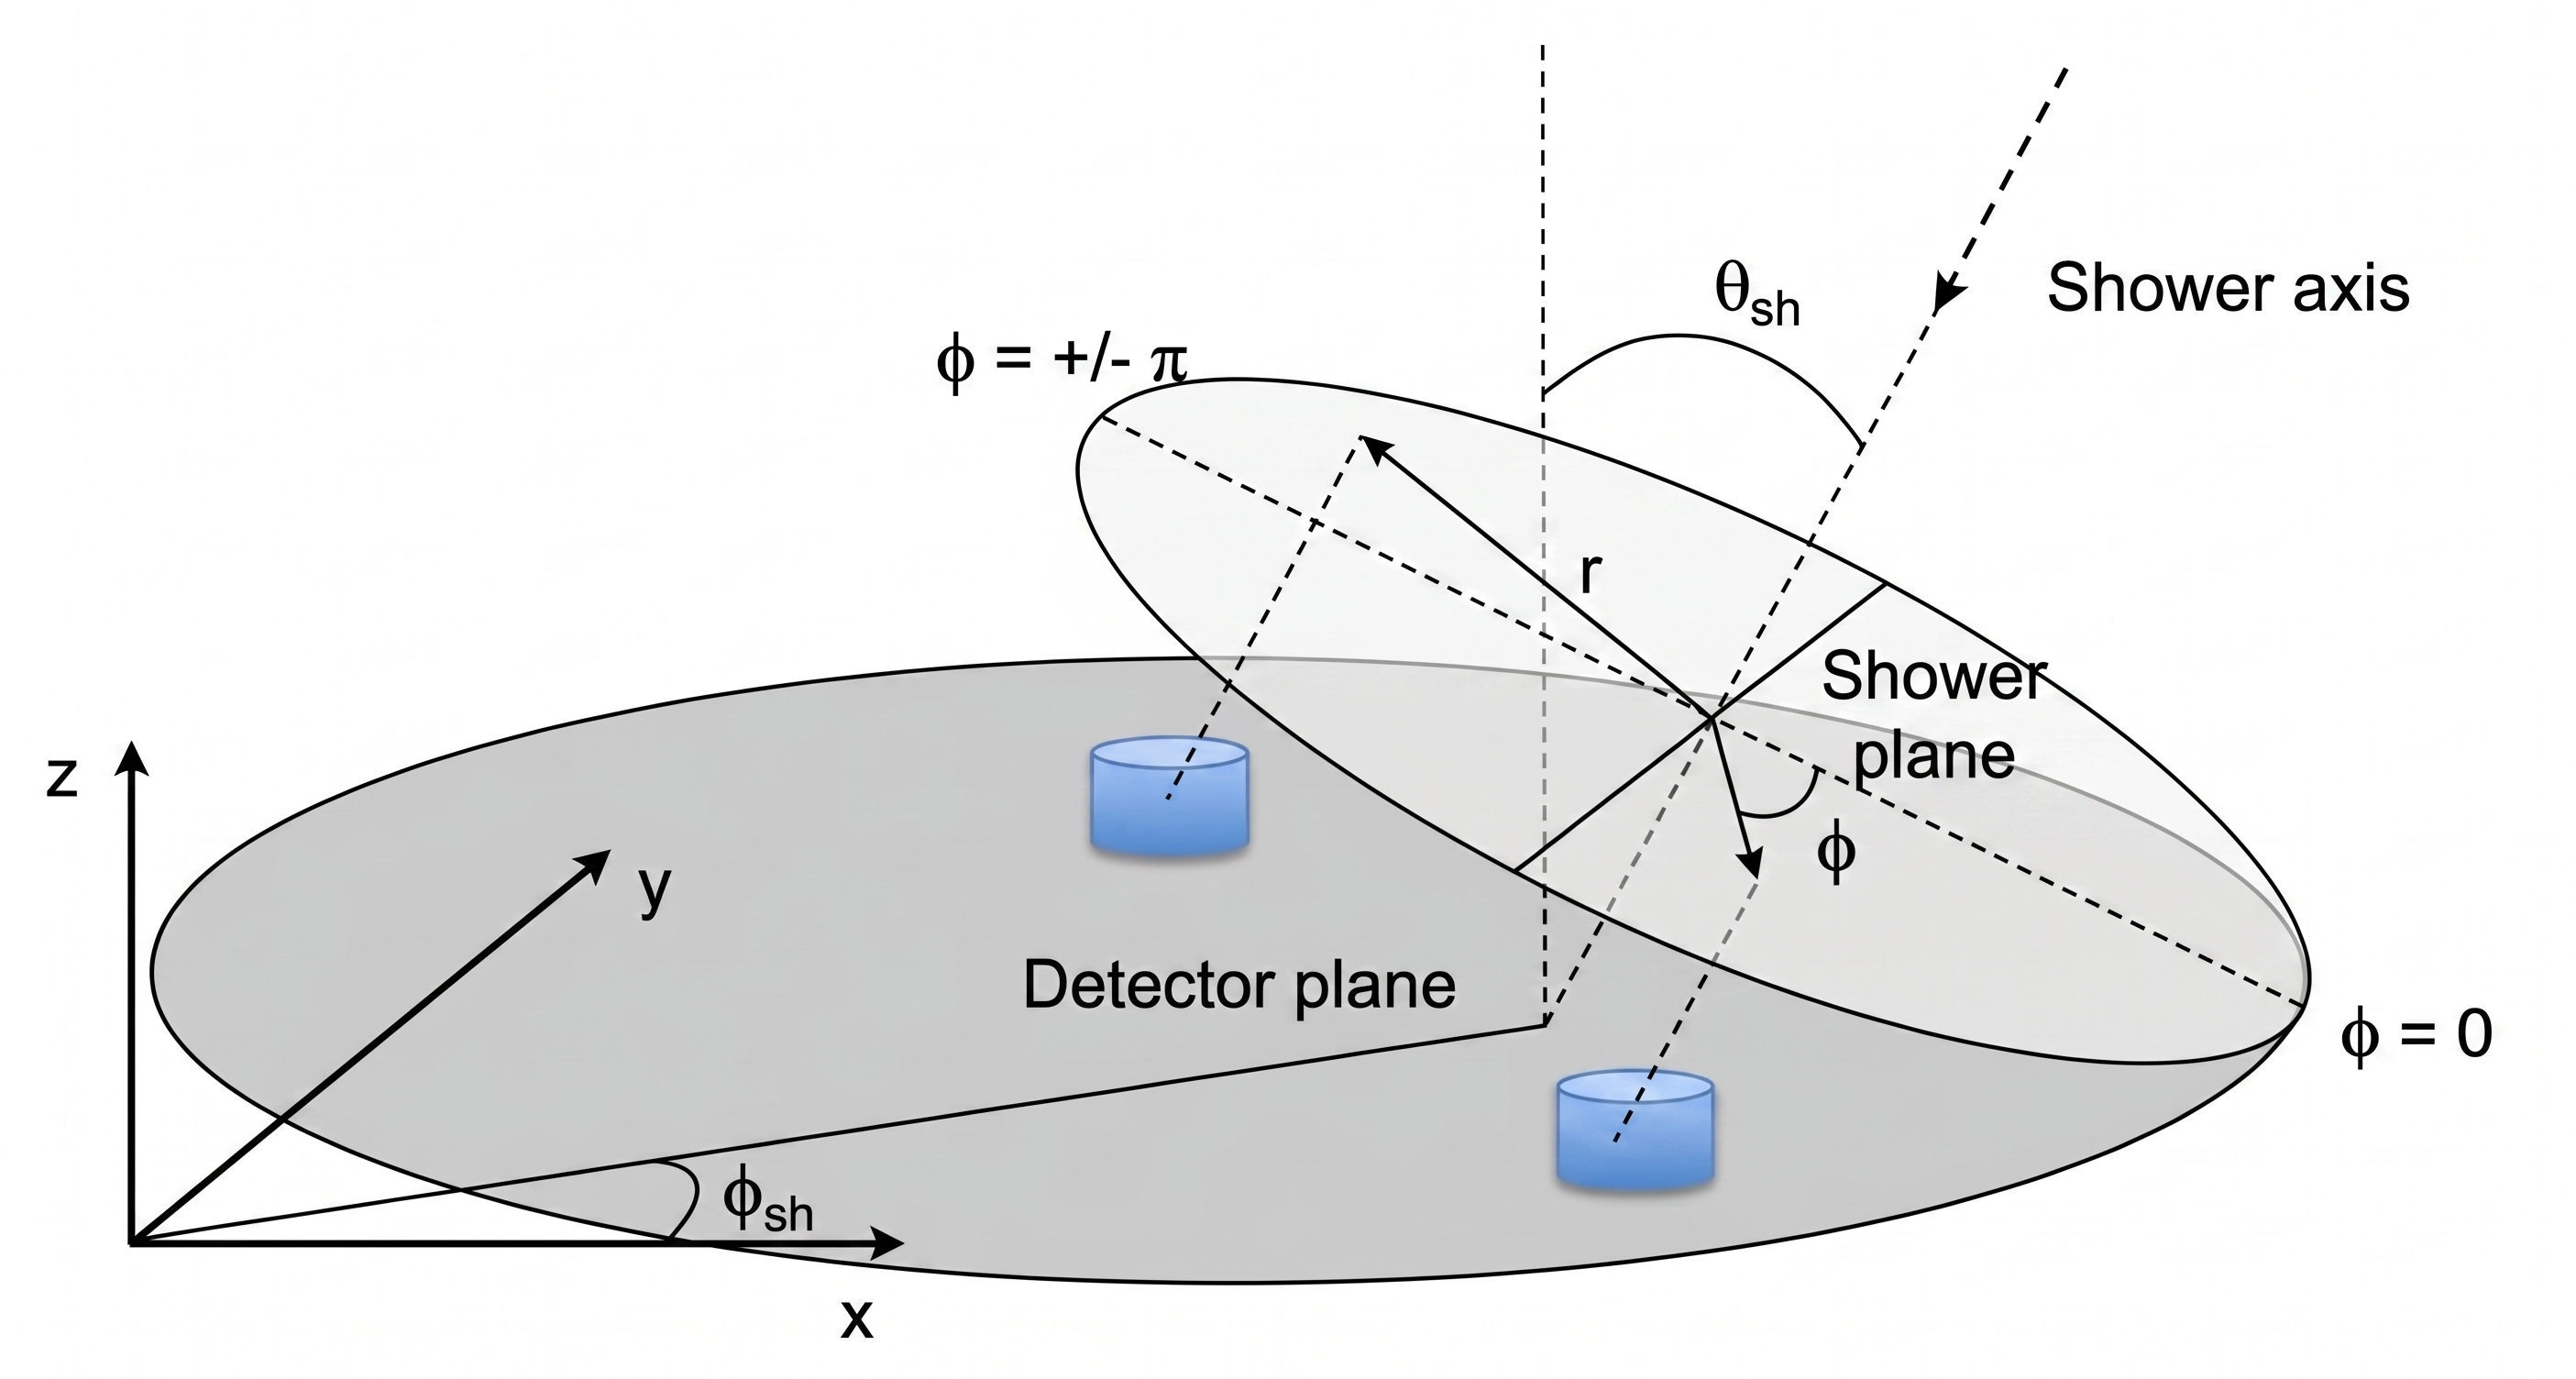
\includegraphics[width=1.08\textwidth]{esquema_lluvia.jpeg}}
  \end{columns}
  \note{%
    The asymmetry of the total SD signal in inclined showers is well known. The
    question here is what happens with muons alone, which is what the UMD gives us:
    shielded, so free of the electromagnetic component. The observable is the
    first-harmonic amplitude A1 of the muon density in the shower plane. For a vertical
    shower the density is circularly symmetric. When the shower is inclined, two regions
    appear: the early side, reached first through less atmosphere, and the late side,
    reached later through more atmosphere. A positive A1 means more muons on the early
    side. A1 is fitted on an ensemble of showers, not event by event.\par
    \textit{Transition:} We start in the cleanest setup we have.}
\end{frame}

% ============================================================
\section{The reference: Monte Carlo geometry}
% ============================================================

\begin{frame}{Simulations and the Dense Ring}
  \begin{columns}[c]
    \column{0.66\textwidth}
      \begin{itemize}
        \item Official CORSIKA + \emph{Offline} production, with SD-750 and UMD:
      \end{itemize}
      \vspace{0.1em}
      {\footnotesize
      \renewcommand{\arraystretch}{1.15}
      \hspace{1.2em}\begin{tabular}{@{}ll@{}}
        \textbf{Hadronic models} & SIBYLL~2.3e (main), QGSJET-III.01, EPOS-LHC-R\\
        \textbf{Primaries} & p, He, O, Fe\\
        \textbf{Energy} & $10^{17.5}$--$10^{18}$~eV\\
        \textbf{Zenith angle} & $\theta\le65^\circ$\\
      \end{tabular}}
      \vspace{0.4em}
      \begin{itemize}
        \item \textbf{Dense Ring}: 12 virtual stations at $r=450$~m from the
          \textbf{true} axis, every $30^\circ$ in the shower plane. Same $r$ for all:
          the radial fall-off of the density cannot produce a modulation in $\phi$.
      \end{itemize}
    \column{0.30\textwidth}
      \centering
      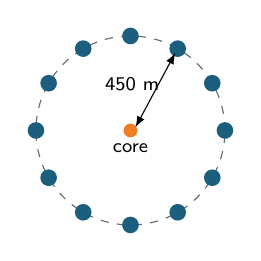
\begin{tikzpicture}[x=0.8cm,y=0.8cm]
        \draw[itedaGray, dashed] (0,0) circle (1.5);
        \foreach \angulo in {0,30,...,330}
          \fill[itedaTeal] (\angulo:1.5) circle (3pt);
        \fill[itedaOrange] (0,0) circle (2.5pt);
        \node[font=\scriptsize, below] at (0,-0.05) {core};
        \draw[{Latex[length=1.4mm]}-{Latex[length=1.4mm]}] (0.08,0.05) -- (60:1.42);
        \node[font=\scriptsize, anchor=east] at (50:0.95) {450 m};
      \end{tikzpicture}

      \vspace{0.3em}
      {\scriptsize Shower plane.}
  \end{columns}
  \note{%
    These are the simulations: the official collaboration production, CORSIKA plus
    Offline, with the 750 meter array and the UMD. Most of what I show is protons with
    SIBYLL 2.3e between ten to the 17.5 and ten to the 18 electronvolts. To isolate the
    effect we start with a synthetic setup, the Dense Ring: twelve virtual stations
    placed in the simulation at 450 meters from the true shower axis, every thirty
    degrees. Since all stations are at the same distance, the steep fall of the
    density with distance cannot produce a modulation in azimuth.\par
    \textit{Transition:} This is what the muon density looks like on the ring.}
\end{frame}

\begin{frame}{A clear modulation on the Dense Ring}
  \badgeAD
  \begin{columns}[c]
    \column{0.60\textwidth}
      \hspace*{-0.5cm}%
      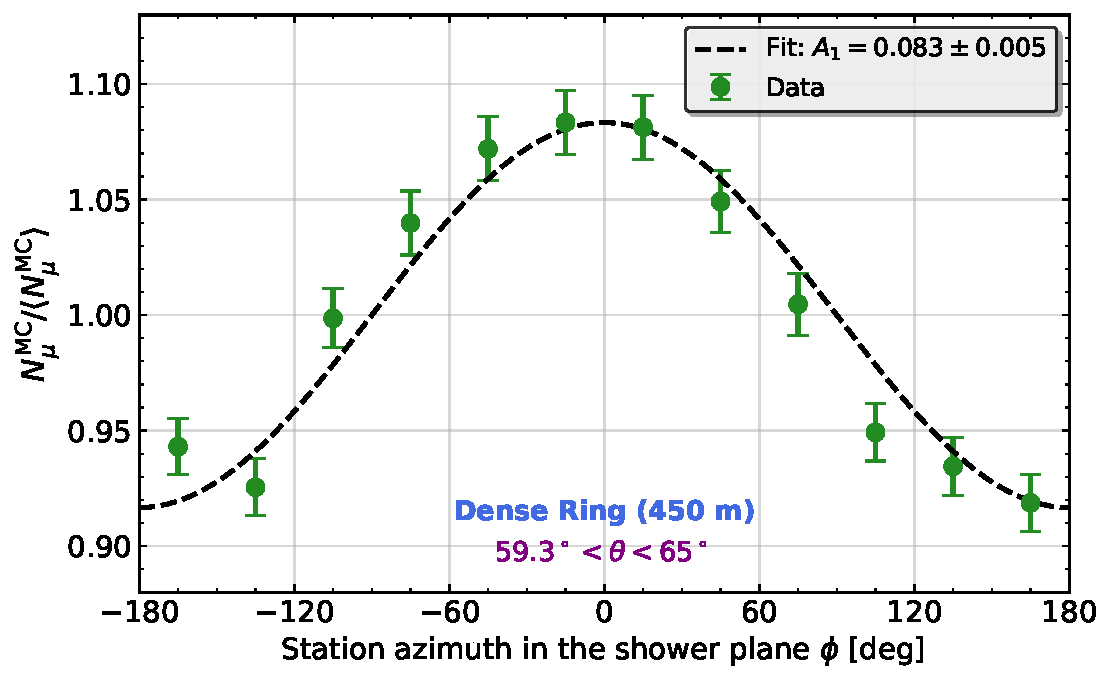
\includegraphics[width=1.04\textwidth,height=6.2cm,keepaspectratio]{DenseRing_Fit_UMD_MC_EN.pdf}
    \column{0.38\textwidth}
      \begin{itemize}
        \item Injected muon number $N_\mu^{\text{MC}}$, $59.3^\circ<\theta<65^\circ$.
        \item Maximum in the \early{} region ($\phi\approx0$).
        \item Early--late difference \alert{$\approx17\%$} peak to peak
          ($\pm8\%$ around the mean).
      \end{itemize}
  \end{columns}
  \note{%
    Here are the twelve ring stations for the most inclined bin, using the injected
    muon numbers. The density peaks on the early side and the first harmonic gives an
    amplitude of 0.083: the early side has about eight percent more muons than the
    mean, the late side eight percent fewer. With the reconstructed muon numbers the
    same bin gives 0.068; that difference is the counting reconstruction, in the
    backup. (If asked: the Dense Ring zenith bins are in reconstructed zenith angle.)\par
    \textit{Transition:} How does it change with zenith angle?}
\end{frame}

\begin{frame}{Comparison: SD vs.\ UMD on the Dense Ring}
  \badgeAD
  \begin{columns}[c]
    \column{0.64\textwidth}
      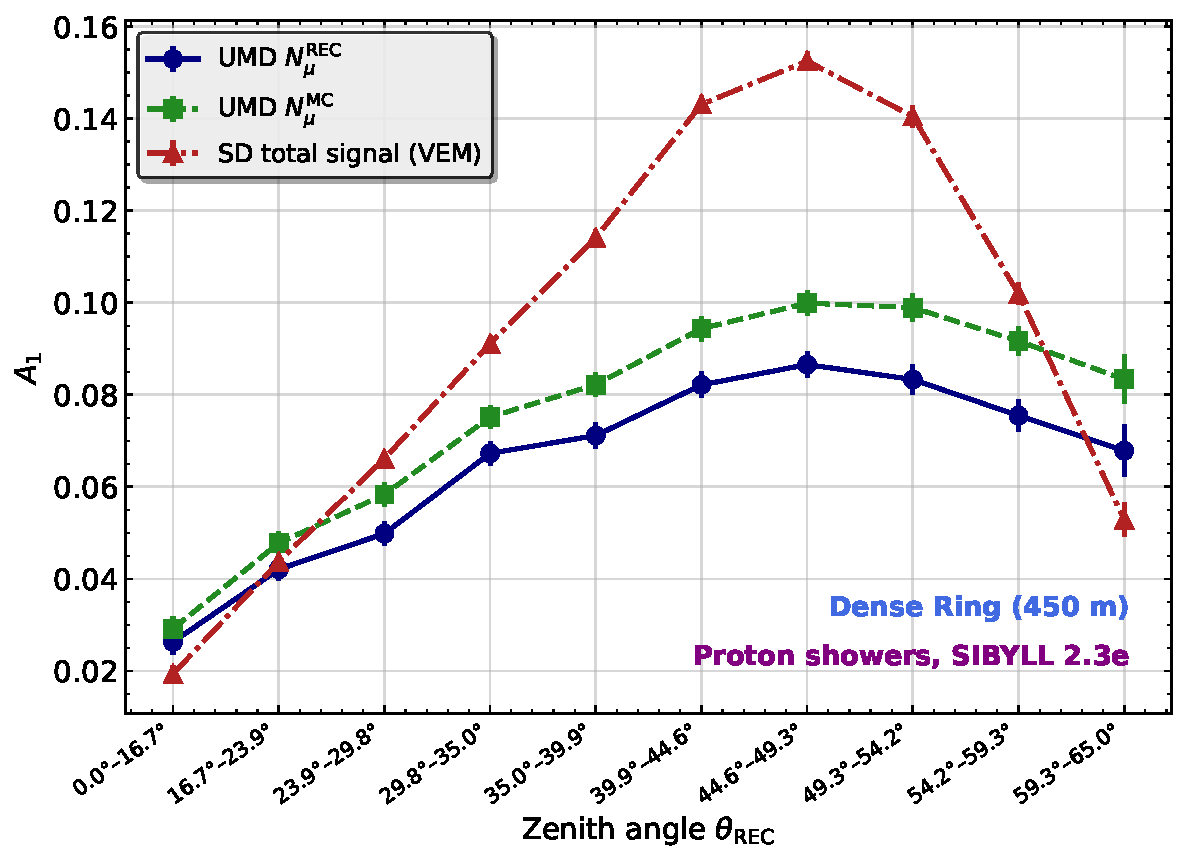
\includegraphics[width=\textwidth]{DenseRing_A1_vs_Theta_EN.pdf}
    \column{0.34\textwidth}
      \footnotesize
      \setbeamerfont{itemize/enumerate body}{size=\footnotesize}
      \begin{itemize}
        \setlength{\itemsep}{2pt}
        \item UMD: $A_1>0$, grows with $\theta$ up to $\sim45$--$50^\circ$.
        \item UMD: lower amplitude with reconstructed ($N_\mu^{\text{REC}}$) than with
          injected ($N_\mu^{\text{MC}}$) muons, same shape.
        \item SD total signal: larger than the UMD at $\sim20$--$60^\circ$
          (EM-dominated); drops sharply above $\sim50^\circ$.
        \item SD below the UMD only at $\theta\gtrsim60^\circ$.
      \end{itemize}
  \end{columns}
  \note{%
    The muon asymmetry is positive and grows with inclination up to about forty-five
    to fifty degrees. The SD total signal is larger over most of the range, because
    it is dominated by the electromagnetic component, which is strongly attenuated
    after the shower maximum. Above about fifty degrees the electromagnetic part is
    mostly absorbed and the SD asymmetry drops quickly; only in the last bin, above
    about sixty degrees, does it fall below the UMD. Note also the gap between the two
    UMD curves: the reconstructed muon numbers give a lower amplitude than the injected
    ones, with the same shape. That comes from the muon-counting reconstruction; it is
    in the backup.\par
    \textit{Transition:} The ring gives us one radius. For the radial dependence we
    need the real Infill array.}
\end{frame}

\begin{frame}{The Infill array: two geometries}
  \badgeIF
  \begin{columns}[c]
    \column{0.57\textwidth}
      \begin{itemize}
        \item Now the real Infill stations (750~m): the distance to the axis varies
          from station to station $\Rightarrow$ we can study $A_1(r)$.
        \item $r$ and $\phi$ of each station depend on where the shower axis is.
          Two geometries:
          \begin{itemize}
            \item \textbf{MC}: true core and direction;
            \item \textbf{REC}: reconstructed core and direction.
          \end{itemize}
        \item The main difference between them is the \textbf{core position}.
      \end{itemize}
    \column{0.40\textwidth}
      \centering
      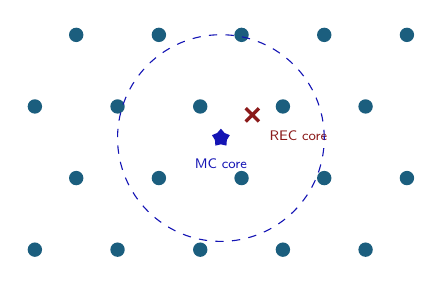
\begin{tikzpicture}[x=1.05cm,y=1.05cm]
        \foreach \fila in {0,1,2,3} {
          \foreach \col in {0,1,2,3,4} {
            \pgfmathsetmacro{\xpos}{\col + 0.5*mod(\fila,2)}
            \pgfmathsetmacro{\ypos}{0.866*\fila}
            \fill[itedaTeal] (\xpos,\ypos) circle (2.6pt);
          }
        }
        \node[star, star points=5, fill=plotBlue, inner sep=1.6pt] at (2.25,1.35) {};
        \node[font=\tiny, plotBlue, anchor=north] at (2.25,1.22) {MC core};
        \draw[plotMaroon, very thick] (2.55,1.55) -- ++(0.16,0.16) (2.55,1.71) -- ++(0.16,-0.16);
        \node[font=\tiny, plotMaroon, anchor=north west] at (2.72,1.55) {REC core};
        \draw[plotBlue, dashed] (2.25,1.35) circle (1.25);
      \end{tikzpicture}

      \vspace{0.2em}
      {\scriptsize Stations every 750~m. With another core, $r$ and $\phi$ of every
      station change.}
  \end{columns}
  \note{%
    Still simulations, but now with the real Infill stations. Their distances to the
    axis vary, so we can follow A1 as a function of r. The distance and azimuth of each
    station depend on where the shower axis is, and there are two choices: the true
    core and direction from the simulation, or the reconstructed ones. The main
    difference between the two is the core position. We start with the true one.\par
    \textit{Transition:} This is the UMD asymmetry with the true geometry.}
\end{frame}

\begin{frame}{UMD radial dependence on the Infill (MC geometry)}
  \badgeIF
  \begin{columns}[c]
    \column{0.62\textwidth}
      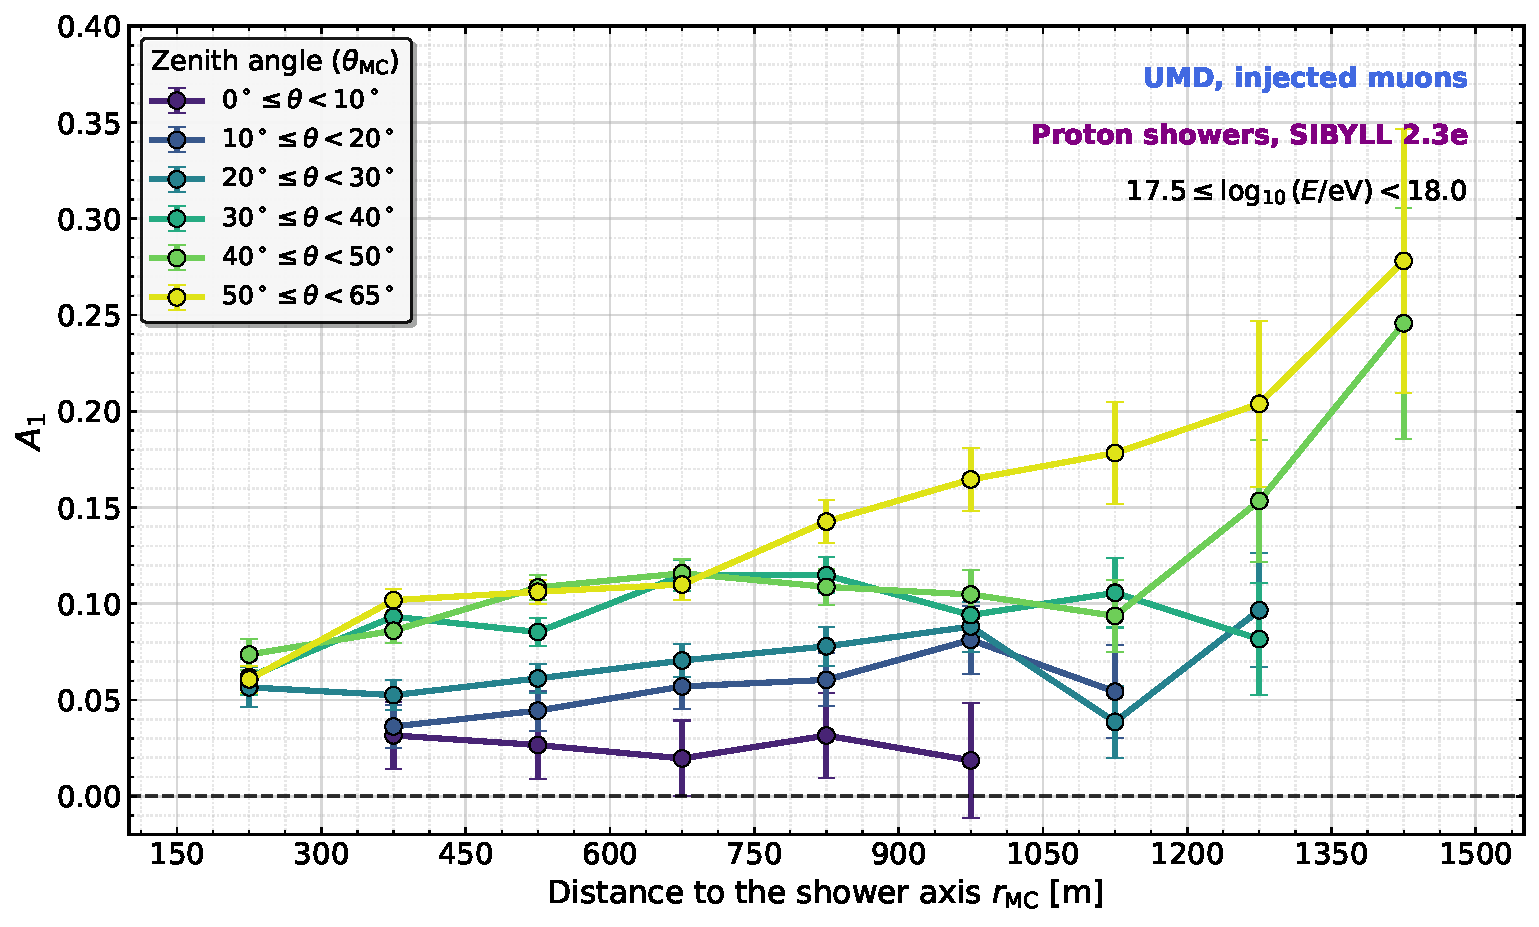
\includegraphics[width=\textwidth]{Infill_UMD_A1_vs_r_MC_EN.pdf}
    \column{0.36\textwidth}
      \footnotesize
      \setbeamerfont{itemize/enumerate body}{size=\footnotesize}
      \begin{itemize}
        \setlength{\itemsep}{2pt}
        \item \textbf{UMD only} (injected muons); $r,\phi$ from the \textbf{true}
          core and direction.
        \item Radial bins of $\Delta r=150$~m; zenith bins of $10^\circ$.
        \item $\theta<10^\circ$: compatible with zero.
        \item $10$--$40^\circ$: grows with $r$, then \textbf{flattens}.
        \item $\theta\ge40^\circ$: \textbf{grows with $r$}.
      \end{itemize}
      \vspace{0.3em}
      \centering\alert{\textbf{This is our reference.}}
  \end{columns}
  \note{%
    This is the UMD alone, with the injected muon numbers and the true core and
    direction, in radial bins of 150 meters and zenith bins of ten degrees. Near-vertical
    showers show no significant asymmetry. Between ten and forty degrees it grows with
    distance and then flattens. Above forty degrees it grows with distance. (If asked:
    at forty to fifty degrees it stays around 0.1 and rises only beyond about twelve
    hundred meters, where the statistics are lower.) This is what an ideal analysis
    should find.\par
    \textit{Transition:} Now we compare with the surface detector in the same
    showers.}
\end{frame}

% ============================================================
\section{The SD inversion and the selection bias}
% ============================================================

\begin{frame}{The SD comparison: inversion far from the core}
  \badgeIF
  \begin{columns}[c]
    \column{0.66\textwidth}
      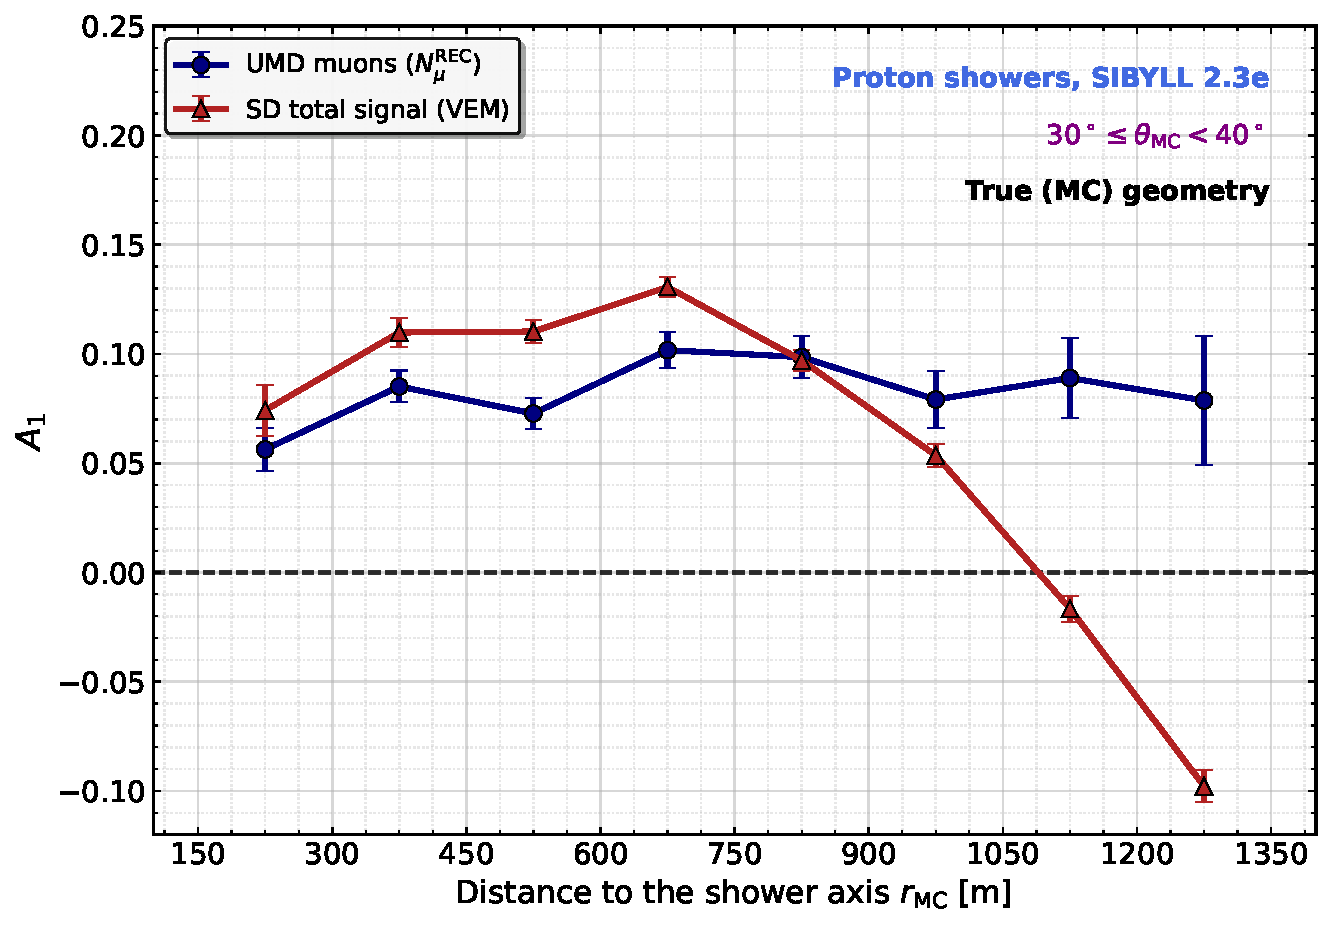
\includegraphics[width=\textwidth]{Infill_UMD_vs_SD_Total_EN.pdf}
    \column{0.32\textwidth}
      \begin{itemize}
        \item We now compare the UMD and SD asymmetries in the same Infill showers.
        \item MC geometry, $30^\circ\le\theta<40^\circ$.
        \item UMD: positive at all $r$.
        \item SD total: a maximum, then \alert{negative} far from the core.
      \end{itemize}
  \end{columns}
  \note{%
    Now we compare the UMD with the surface detector, on the same Infill showers and
    with the same true geometry. The UMD stays positive at all distances. The total SD
    signal peaks, then decreases, and far from the core becomes clearly negative, an
    excess on the late side. Since the core and direction are the true ones, this
    cannot be a reconstruction error.\par
    \textit{Transition:} Which part of the tank signal is responsible?}
\end{frame}

\begin{frame}[t]{It is the SD muon component that inverts}
  \badgeIF
  \vspace{-0.6em}
  \begin{columns}[T]
    \column{0.62\textwidth}
      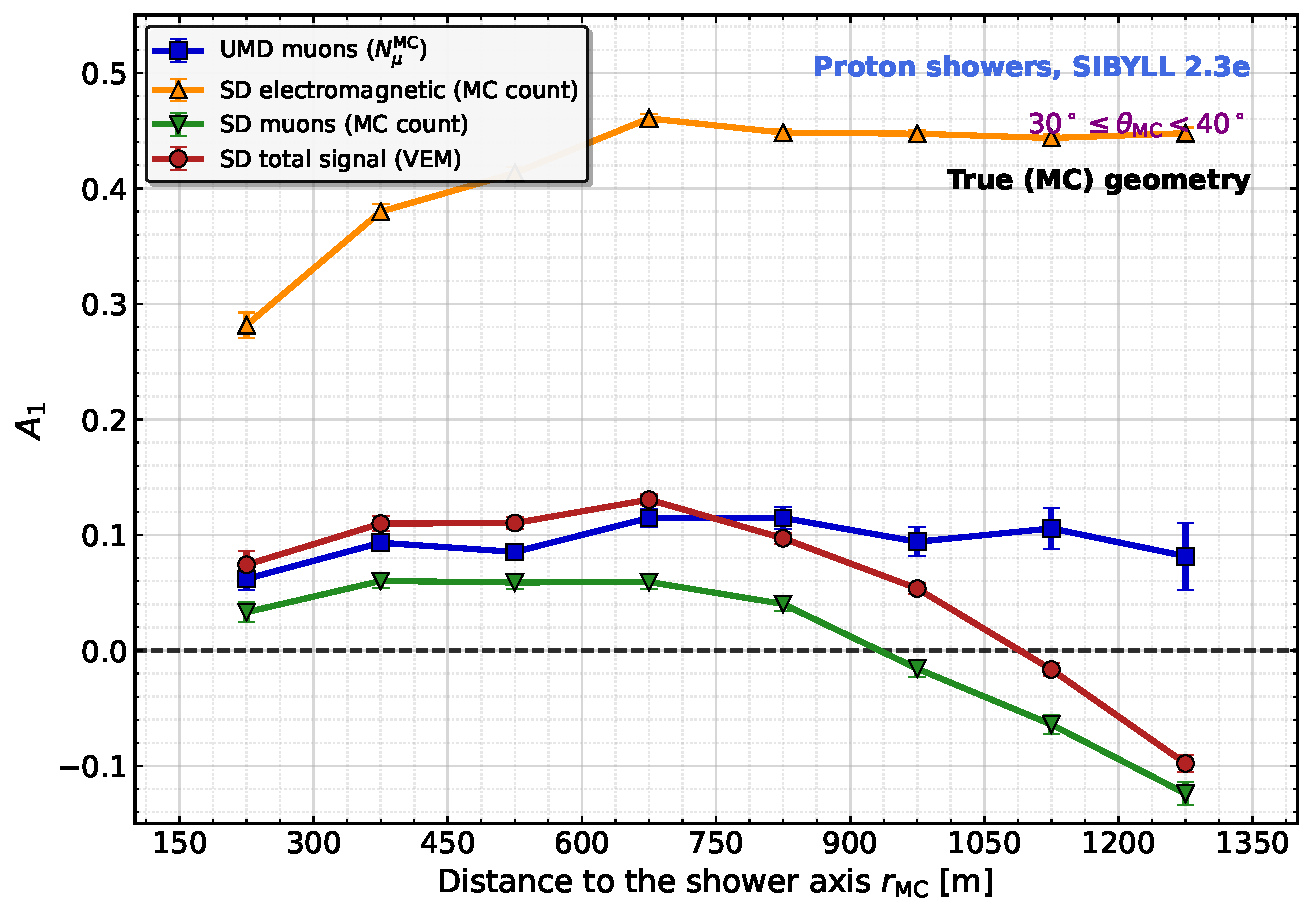
\includegraphics[width=\textwidth]{Infill_SD_Breakdown_vs_UMD_EN.pdf}
    \column{0.36\textwidth}
      \begin{itemize}
        \item MC particle counts in the tank, split by component.
        \item \textcolor{itedaOrange}{\textbf{EM}}: positive at all $r$.
        \item \textcolor{plotGreen}{\textbf{SD muons}}: positive near the core,
          \alert{negative} beyond $\sim900$~m.
        \item The SD total follows its muons at large $r$.
      \end{itemize}
      \vspace{0.3em}
      \centering\alert{\textbf{Same quantity, opposite sign in UMD and SD.}}
  \end{columns}
  \note{%
    Splitting the tank signal with the simulation truth, the electromagnetic part is
    positive everywhere. The muon part is what inverts, and the total SD signal
    follows it far from the core. So we compare the same physical quantity, muons
    crossing a detector, and get opposite signs in the UMD and in the SD. Our
    analytic model of muon propagation does not produce a negative asymmetry at these
    distances, so we looked at how the observable is built.\par
    \textit{Transition:} The key point: we never average over all stations.}
\end{frame}

\begin{frame}{Hypothesis: the station selection biases the average}
  \badgeHYP
  \small
  A station enters the analysis only if it \textbf{belongs to the reconstructed
  event} (\texttt{HasStation}). If the probability that a station is kept depends on
  its own muon content, and this dependence is not the same on the early and late
  sides, the \textbf{regional averages are biased}.
  \vspace{0.3em}
  \begin{center}
  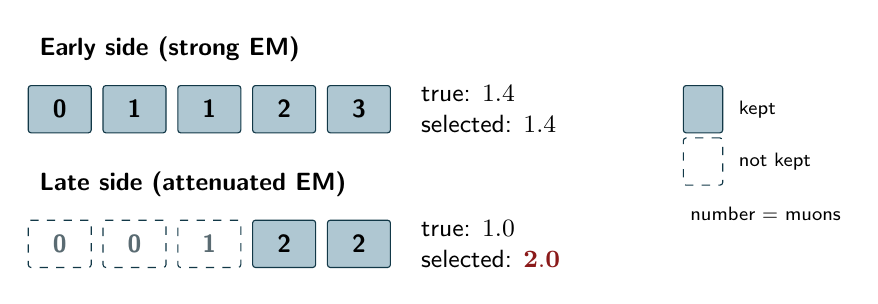
\begin{tikzpicture}[x=0.95cm,y=0.95cm,
      tank/.style={draw=itedaTealDark, minimum width=0.8cm, minimum height=0.6cm, rounded corners=1pt, font=\small\bfseries},
      on/.style={tank, fill=itedaTeal!35},
      off/.style={tank, fill=white, dashed, text=itedaGray}]
    \node[font=\small\bfseries, anchor=west] at (-0.4,1.2) {Early side (strong EM)};
    \foreach \x/\n in {0/0,1/1,2/1,3/2,4/3} {\node[on] at (\x,0.4) {\n};}
    \node[font=\small, anchor=west, align=left] at (4.7,0.4) {true: $1.4$\\ selected: $1.4$};
    \node[font=\small\bfseries, anchor=west] at (-0.4,-0.6) {Late side (attenuated EM)};
    \foreach \x/\n in {0/0,1/0,2/1} {\node[off] at (\x,-1.4) {\n};}
    \foreach \x/\n in {3/2,4/2} {\node[on] at (\x,-1.4) {\n};}
    \node[font=\small, anchor=west, align=left] at (4.7,-1.4) {true: $1.0$\\ selected: \textcolor{plotMaroon}{$\mathbf{2.0}$}};
    \node[on, minimum width=0.5cm] at (8.6,0.4) {};
    \node[font=\scriptsize, anchor=west] at (8.95,0.4) {kept};
    \node[off, minimum width=0.5cm] at (8.6,-0.3) {};
    \node[font=\scriptsize, anchor=west] at (8.95,-0.3) {not kept};
    \node[font=\scriptsize, anchor=west] at (8.3,-1.0) {number = muons};
  \end{tikzpicture}
  \end{center}
  \vspace{-0.2em}
  \centering The sign can flip \textbf{without moving a single muon}.
  \fuente{Illustrative cartoon, not simulation output.}
  \note{%
    Every curve so far is an average over stations that are part of the reconstructed
    event. For the UMD that seemed natural, since it has no trigger of its own. But
    suppose the chance that a station is kept depends on how many muons it has. On
    the early side the electromagnetic signal is strong enough that almost every
    station is kept. On the late side it is more attenuated, so mostly the stations
    with more muons survive. The late average is pulled up, and the asymmetry can
    change sign although no muon was created or moved. This is a hypothesis; the next
    two slides test it.\par
    \textit{Transition:} The direct test is to remove the requirement.}
\end{frame}

\begin{frame}{Test 1: without \texttt{HasStation}, the inversion disappears}
  \badgeIF
  \vspace{-0.8em}
  \begin{columns}[c]
    \column{0.62\textwidth}
      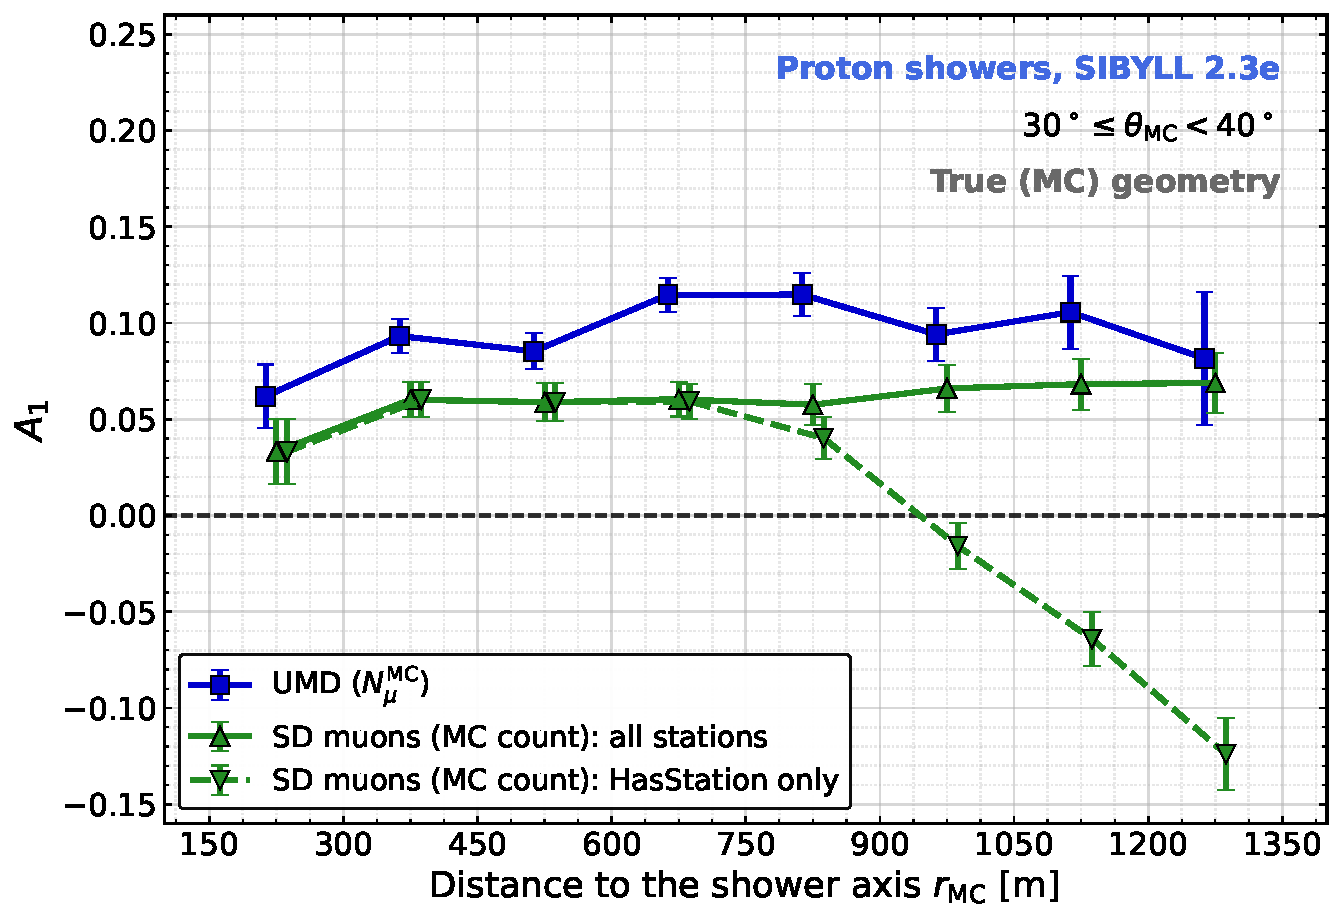
\includegraphics[width=\textwidth]{Selection_Test1_EN.pdf}
    \column{0.36\textwidth}
      \begin{itemize}
        \item Same MC counts, coordinates and fit: only \textbf{which stations}
          enter changes.
        \item All stations: SD muons \textbf{positive at all $r$}
          ($+0.03$ to $+0.07$).
        \item Same sign and trend as the UMD, \textbf{but not the same values}.
      \end{itemize}
  \end{columns}
  \note{%
    Same Monte Carlo muon counts in the tanks, same coordinates, same fit; only which
    stations enter changes. Over all simulated stations the SD muon asymmetry is
    positive at all distances, between plus three and plus seven percent. Requiring
    the station to be in the reconstructed event changes nothing up to about 750
    meters, where practically every station is kept, and then drives the asymmetry
    down to minus 0.12 at twelve to thirteen hundred meters: plus 0.069 plus or minus
    0.016 over all stations, against minus 0.124 plus or minus 0.019 with the
    requirement. The errors come from a bootstrap over the 960 showers, keeping the
    stations of each shower together. So the sign flip is a
    property of the station sample. Without the selection the SD muons have the same
    sign and trend as the UMD, but between 150 and 900 meters the UMD is still 0.03 to
    0.06 higher; detector response and threshold are candidates, this is open.\par
    \textit{Transition:} If this is a trigger effect, there is a direct check.}
\end{frame}

\begin{frame}[t]{Test 2: the excluded tanks should hold very few muons}
  \badgeIF
  \vspace{-1.5em}
  \footnotesize
  \setbeamerfont{itemize/enumerate body}{size=\footnotesize}
  \begin{itemize}
    \setlength{\itemsep}{1pt}
    \item If the inversion comes from the \textbf{trigger}, the tanks dropped by the
      reconstruction (\texttt{HasStation} = False) should have been crossed, on average,
      by \alert{at most one muon}, too few for the station to trigger.
    \item Excluded tanks: $\le1\,\mu$ in \alert{95\%} (early) and \alert{93\%} (late) of
      the cases.
  \end{itemize}
  \vspace{0.1em}
  \centering
  \makebox[\textwidth][c]{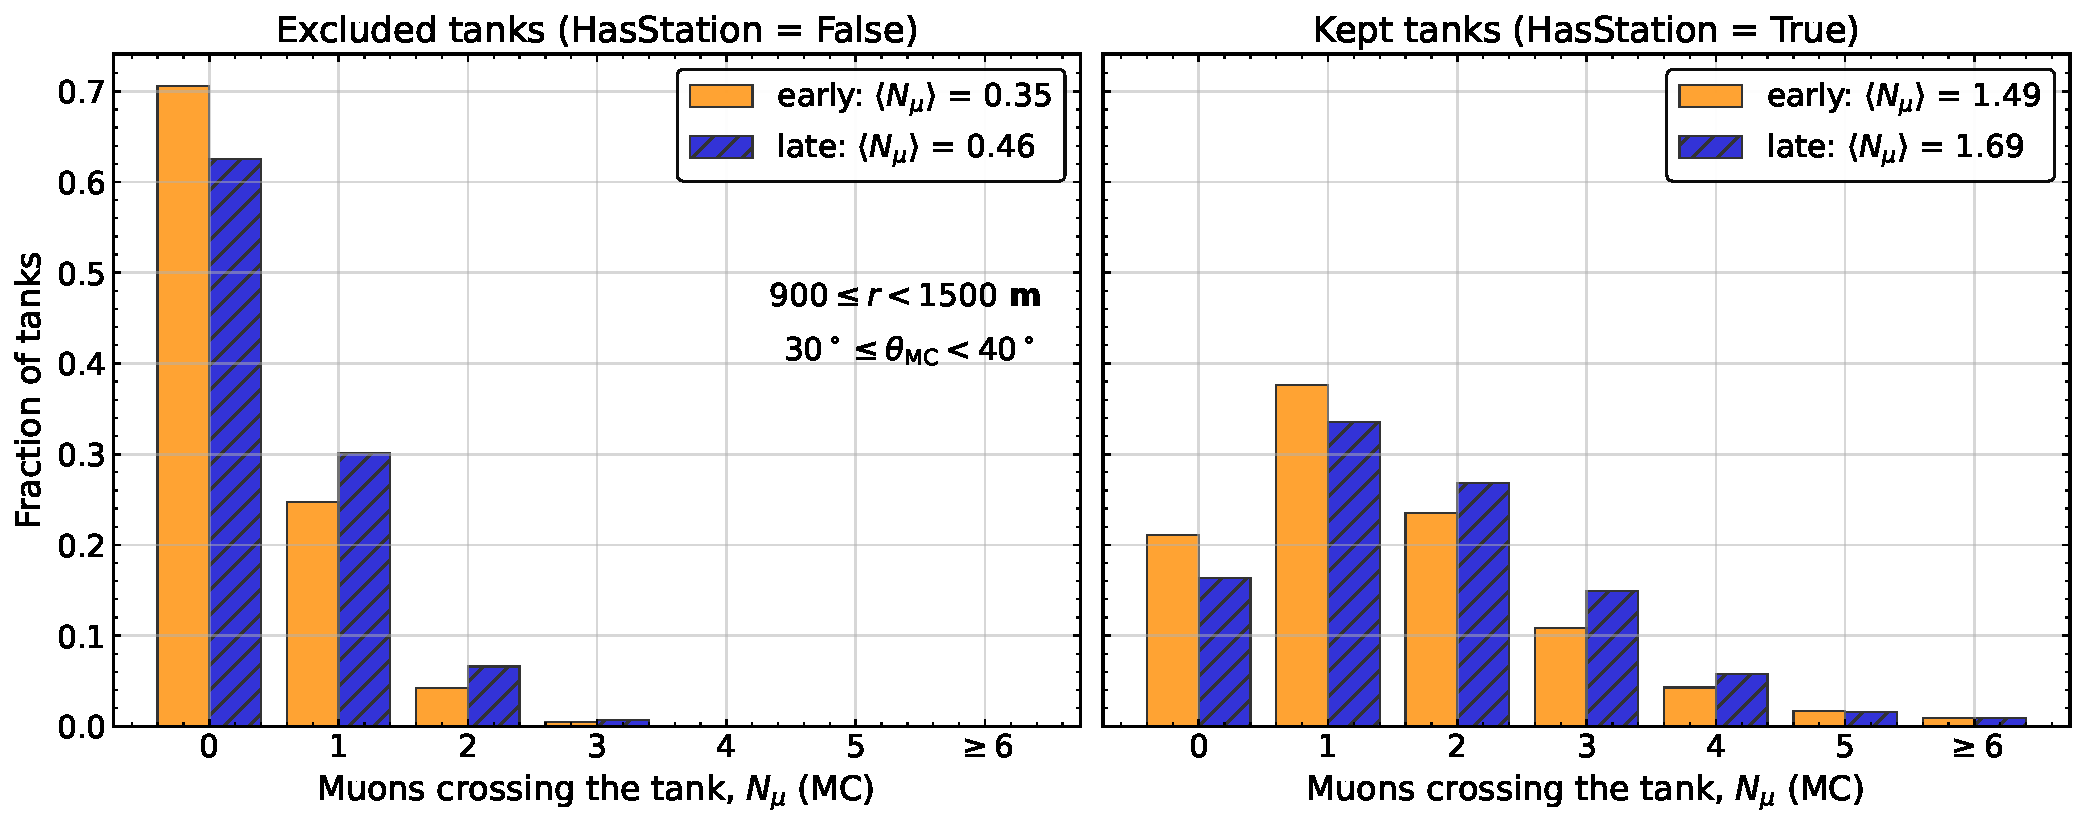
\includegraphics[width=1.04\textwidth,height=4.9cm,keepaspectratio]{Selection_Test2_EN.pdf}}
  \note{%
    If the inversion is a trigger effect, there is a clear prediction: the tanks that
    the reconstruction drops should have been crossed by at most about one muon. If we
    found excluded tanks with several muons, a trigger explanation would not be
    credible. So we count the Monte Carlo muons in the excluded tanks. Ninety-five
    percent of the excluded early tanks and ninety-three percent of the late ones have
    at most one muon. The excluded late tanks have about half the electromagnetic
    particles of the early ones, 14 against 28, so on the late side we lose tanks that
    on the early side would have been kept thanks to their electromagnetic signal. That
    is why, among the kept tanks, the late ones carry more muons than the early ones,
    even though the true density is higher on the early side, and why only eighteen
    percent of the late stations are kept far from the core, against forty-two percent
    of the early ones. This supports the trigger picture, but HasStation also includes
    readout and reconstruction, and we have not separated them, so it is consistent
    with a trigger effect, not a proof. (Early: $|\phi|<60^\circ$, late: $|\phi|>120^\circ$;
    MC geometry.)\par
    \textit{Transition:} So far, true core and direction. In real data we only have the
    reconstructed ones.}
\end{frame}

% ============================================================
\section{Reconstructed geometry and the core position}
% ============================================================

\begin{frame}[t]{With REC geometry, the UMD asymmetry vanishes}
  \badgeIF
  \vspace{-0.6em}
  \begin{itemize}
    \item Same UMD modules, same \textbf{injected} muon number, $450\le r<600$~m.
  \end{itemize}
  \begin{center}
    \renewcommand{\arraystretch}{1.15}
    \begin{tabular}{lcc}
      \toprule
      $\theta$ & $A_1$ Monte Carlo & $A_1$ Reconstructed\\
      \midrule
      $20^\circ$--$30^\circ$ & $0.062$ & $0.011$\\
      $30^\circ$--$40^\circ$ & $0.086$ & $0.002$\\
      $40^\circ$--$50^\circ$ & $0.108$ & \textcolor{plotMaroon}{$-0.002$}\\
      \bottomrule
    \end{tabular}
  \end{center}
  \begin{itemize}
    \item With the \textbf{reconstructed core}, the asymmetry is lost almost completely.
    \item The effect comes from the \textbf{offset between the true and the reconstructed
      core positions}.
  \end{itemize}
  \note{%
    Same UMD modules, same injected muon numbers; we only change the geometry used to
    compute each station's distance and azimuth. With the reconstructed core the
    asymmetry essentially disappears: at forty to fifty degrees it goes from 0.108 to
    zero. We also swapped the two quantities one at a time: using the reconstructed or
    the true azimuth gives the same A1 within 0.002, so everything comes from the
    distance to the reconstructed core. (If asked: farther out, at forty to fifty degrees
    and 600 to 1050 meters, the asymmetry survives but reduced, below 0.05 against about
    0.11.)\par
    \textit{Transition:} So where is the reconstructed core?}
\end{frame}

\begin{frame}[t]{The reconstructed core is shifted toward the early region}
  \badgeIF
  \vspace{-1.2em}
  \centering
  \makebox[\textwidth][c]{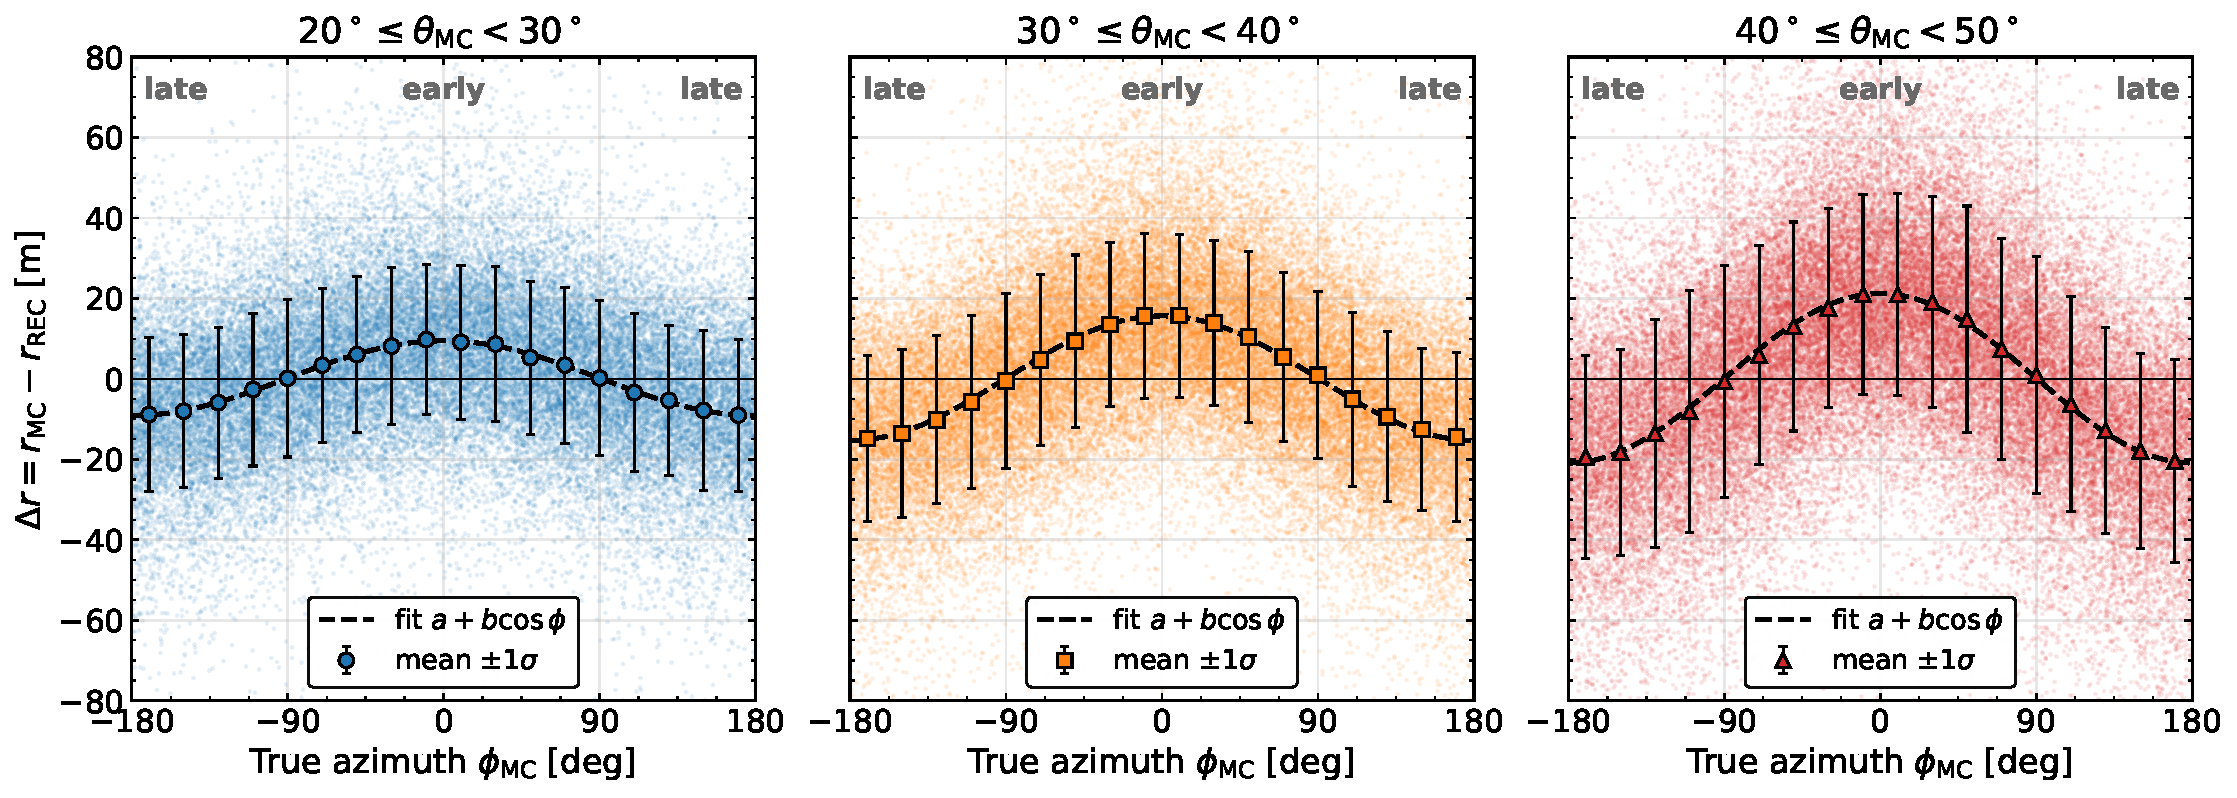
\includegraphics[width=1.06\textwidth,height=5.0cm,keepaspectratio]{Core_Shift_EN.pdf}}

  \vspace{0.1em}
  \raggedright
  \footnotesize
  \setbeamerfont{itemize/enumerate body}{size=\footnotesize}
  \begin{itemize}
    \setlength{\itemsep}{0pt}
    \item $\Delta r=r_{\text{MC}}-r_{\text{REC}}$ vs.\ $\phi$ can be fitted by
      $a+b\cos\phi$: early stations are placed \textbf{closer} to the core, late ones
      \textbf{farther}, with $b\simeq9$, $15$, $21$~m, increasing with $\theta$.
    \item Likely cause: the reconstruction LDF is \textbf{symmetric in $\phi$}; it absorbs
      the early excess by \textbf{moving the core toward the early side, where there is
      more signal}.
  \end{itemize}
  \note{%
    For each station we compare its distance to the true and to the reconstructed
    core, as a function of its true azimuth. If the core error were random, this
    would be flat. Instead it follows a cosine: early stations are placed closer to
    the core than they are, late stations farther. That is the signature of a
    systematic shift of the reconstructed core toward the early side, by about nine,
    fifteen and twenty-one meters in these three zenith bins. A likely reason: the LDF
    used in the reconstruction is symmetric in azimuth. Faced with more signal on the
    early side, the only thing the fit can do is move the core toward it. (Infill
    stations with reconstructed distance below 1400 meters.)\par
    \textit{Transition:} What does a shift of this size do to the LDF, and to A1?}
\end{frame}

\begin{frame}{A shifted core adds a $\cos\phi$ term to the LDF}
  \badgeIF
  \vspace{-0.6em}
  \begin{itemize}
    \item Approximating the LDF locally as $\rho\propto r^{-\beta}$ and correcting it
      for the core shift with an azimuthal dependence, $r\to r+b\cos\phi$:
      \begin{equation*}
        \rho(r+b\cos\phi)\simeq\rho(r)\Big[1-\beta\,\frac{b}{r}\cos\phi\Big]
        \;\Rightarrow\;\boxed{\Delta A_1\simeq-\beta\,\frac{b}{r}}
      \end{equation*}
  \end{itemize}
  \centering
  \renewcommand{\arraystretch}{1.08}
  \begin{tabular}{lcccc}
    \toprule
    $\theta$ & $A_1$ (MC) & $A_1$ (REC) & $\Delta A_1$ &
    \textbf{$A_1^{\text{REC}}+\beta b/r$}\\
    \midrule
    $20$--$30^\circ$ & $0.062$ & $0.011$  & $-0.051$ & $\mathbf{0.062}$\\
    $30$--$40^\circ$ & $0.086$ & $0.002$  & $-0.084$ & $\mathbf{0.083}$\\
    $40$--$50^\circ$ & $0.108$ & $-0.002$ & $-0.110$ & $\mathbf{0.100}$\\
    \bottomrule
  \end{tabular}

  \vspace{0.4em}
  \raggedright
  \begin{itemize}
    \item The shift accounts for \textbf{93--100\%} of the loss; adding it back
      \textbf{recovers the MC reference asymmetry} to $\lesssim0.01$.
  \end{itemize}
  \fuente{$450\le r<600$~m, injected muons. $\beta=2.9,\,2.7,\,2.5$ (UMD muon LDF, same simulations).
    Last column derived from the table.}
  \note{%
    Locally the muon LDF falls as a power law with slope beta, between about 2.4 and
    2.9 at these distances. If the reconstructed core is shifted by b toward the early
    side, a station we place at distance r on the early side is really at r plus b,
    so it has fewer muons than we think, and a late station has more. To first order
    this multiplies the LDF by one minus beta b over r times cos phi: a cosine
    modulation with the opposite sign to the physical one. So the reconstructed
    asymmetry should be lower by beta b over r. The prediction, minus 0.051, 0.081 and
    0.102, matches the observed loss in the three zenith bins. Read the other way: adding beta b over r back to
    the reconstructed value recovers the Monte Carlo reference within about 0.01.
    The exact agreement depends on the beta fit range and on the effective r of the
    bin at the ten percent level.\par
    \textit{Transition:} So what would it take to apply this to real data?}
\end{frame}

\begin{frame}{Recovering the asymmetry: what it needs, what is missing}
  \badgeIF
  \vspace{-0.6em}
  \footnotesize
  \setbeamerfont{itemize/enumerate body}{size=\footnotesize}
  \begin{columns}[T]
    \column{0.49\textwidth}
      \begin{block}{What the correction needs}
        \footnotesize
        \begin{itemize}
          \setlength{\itemsep}{0pt}
          \item $b(\theta)$: mean core shift, early--late direction.
            \alert{Measured with MC truth.}
          \item $\beta$: local slope of the muon LDF. From MC here; in principle
            measurable in data.
          \item Apply: move the core back by $b$, or add $\beta b/r$ to $A_1$.
        \end{itemize}
      \end{block}
      \begin{block}{Established}
        \footnotesize
        The loss is \textbf{systematic}, not resolution, and predicted by
        $\beta b/r$ ($450$--$600$~m, $20$--$50^\circ$).
      \end{block}
    \column{0.49\textwidth}
      \begin{alertblock}{Not done yet}
        \footnotesize
        \begin{itemize}
          \setlength{\itemsep}{0pt}
          \item Move the core and recompute $A_1(r)$ at all $r$.
          \item Counting bias ($N_\mu^{\text{REC}}$, 5--23\%): separate effect.
          \item \textbf{For data} (no true core), $b$ must come from:
            \begin{itemize}
              \setlength{\itemsep}{0pt}
              \item $b(\theta)$ parametrized on simulations and \textbf{validated on
                unseen ones} (other showers, primaries, models; tested so far: p,
                SIBYLL~2.3e);
              \item or an LDF fit with an azimuthal term in the reconstruction.
            \end{itemize}
        \end{itemize}
      \end{alertblock}
  \end{columns}
  \note{%
    The correction has two ingredients. The slope beta is a property of the lateral
    distribution and could in principle be measured from the data themselves. The
    shift b is the delicate part: so far we measure it against the true core, which
    only exists in simulations. In data there is no true core, so there are two ways.
    One is to parametrize b as a function of zenith angle on one set of simulations and
    check, as in a train and test split, that it recovers the asymmetry on simulations
    it has not seen: other showers, other primaries, other hadronic models. That tells
    us how model- and composition-dependent the correction is; it does not test the
    differences between data and simulations, such as the muon deficit. The other way is
    to remove the shift at its origin, with a reconstruction LDF that allows an
    azimuthal modulation. At Infill energies the
    station multiplicity makes that hard event by event, but it is worth trying for
    the most energetic events. The test is done in one radial bin, for protons with
    one hadronic model, and with injected muon numbers. The counting bias of the UMD
    reconstruction is a separate, smaller effect.\par
    \textit{Transition:} Let me summarize.}
\end{frame}

% ============================================================
\section{Conclusions}
% ============================================================

\begin{frame}{Conclusions}
  \small
  \begin{enumerate}
    \setlength{\itemsep}{0.45em}
    \item In simulations the UMD muon density has a \textbf{positive early--late
      asymmetry}: it grows with $r$ for inclined showers and is roughly flat at
      intermediate angles.
    \item The SD muon asymmetry inverts far from the core \textbf{only} when averaging
      over the stations kept by the reconstruction: the selection acts \textbf{station by
      station}, not shower by shower. Over all stations it is positive. The excluded
      tanks hold \textbf{mostly} $\le1$ muon: \textbf{consistent with} a trigger effect,
      not yet proven.
    \item With the reconstructed geometry the UMD asymmetry nearly vanishes near the
      core: the reconstructed core is shifted toward the early region by
      $b\approx9$--$21$~m.
    \item This loss follows $\Delta A_1\simeq-\beta\,b/r$; adding it back recovers the
      MC reference. Applying it to data requires $b$ \textbf{without MC truth}.
  \end{enumerate}
  \vspace{0.4em}
  \centering\alert{\textbf{Data--MC comparisons need the same station selection and the
  same geometry.}}
  \note{%
    Four points. The muon asymmetry is there, and it behaves as expected with zenith
    angle and distance. What we measure depends on how we build the observable: which
    stations we average over can flip the sign, and the reconstructed core can erase
    it. The second effect is simple and predictable, so it can be accounted for, and
    any comparison between data and simulation must use the same station selection
    and geometry. The open step is to determine the core shift without Monte Carlo
    truth.}
\end{frame}

\begin{frame}{Next steps}
  \begin{itemize}
    \setlength{\itemsep}{0.4em}
    \item Parametrize the correction parameters vs.\ zenith angle: $b(\theta)$ and
      $\beta(\theta)$, at fixed energy ($17.5\le\lg E<18.0$), and validate the recovery
      on independent simulations.
    \item Apply the full correction (core shift + LDF term) over the whole radial
      range and compare with the MC reference.
    \item Dependence on primary and hadronic model.
    \item Separate trigger, readout and reconstruction inside \texttt{HasStation}.
    \item Apply to field data.
  \end{itemize}
  \note{%
    The natural next step is to parametrize b and beta as functions of zenith angle,
    so that the correction can be applied without a per-bin Monte Carlo comparison.
    Our sample covers a single energy range, so this is a zenith-angle
    parametrization only, not an energy one.}
\end{frame}

\begin{frame}[plain]
  \begin{tikzpicture}[remember picture, overlay]
    \node[anchor=center, inner sep=0pt] at (current page.center)
      {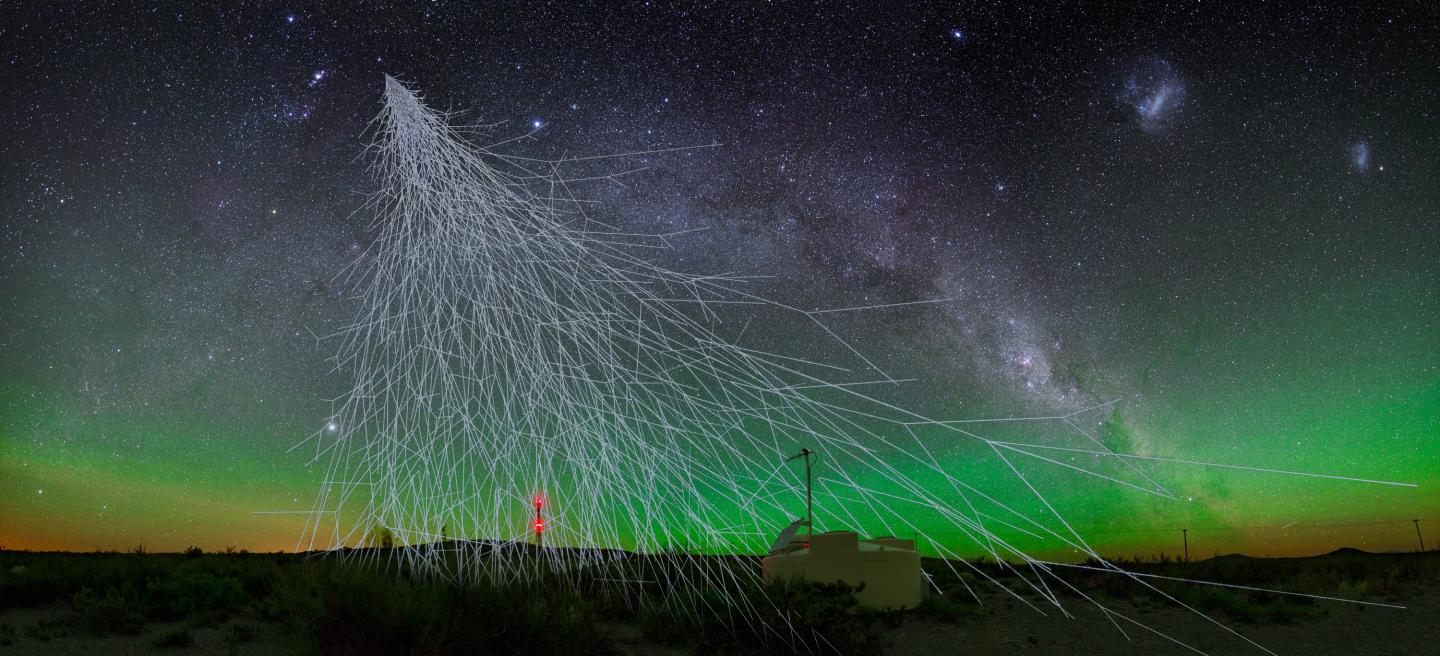
\includegraphics[height=\paperheight]{auger_cr.jpg}};
    \node[anchor=north east, xshift=-0.86cm, yshift=-0.49cm, text=black, opacity=0.6,
      font=\fontsize{34}{38}\selectfont\bfseries] at (current page.north east) {Thank you!};
    \node[anchor=north east, xshift=-0.9cm, yshift=-0.45cm, text=white,
      font=\fontsize{34}{38}\selectfont\bfseries] at (current page.north east) {Thank you!};
    \node[anchor=north east, xshift=-0.91cm, yshift=-1.79cm, text=black, opacity=0.6,
      font=\LARGE\bfseries] at (current page.north east) {Questions?};
    \node[anchor=north east, xshift=-0.95cm, yshift=-1.75cm, text=itedaOrange,
      font=\LARGE\bfseries] at (current page.north east) {Questions?};
    \node[anchor=south east, xshift=-0.15cm, yshift=0.1cm, text=white, opacity=0.8,
      font=\tiny] at (current page.south east)
      {Image: A.~Chantelauze, S.~Staffi, L.~Bret (Pierre Auger Observatory)};
  \end{tikzpicture}
\end{frame}

% ============================================================
\appendix
% ============================================================

\begin{frame}{Backup: muon-counting reconstruction (MC geometry)}
  \badgeIF
  \begin{columns}[c]
    \column{0.60\textwidth}
      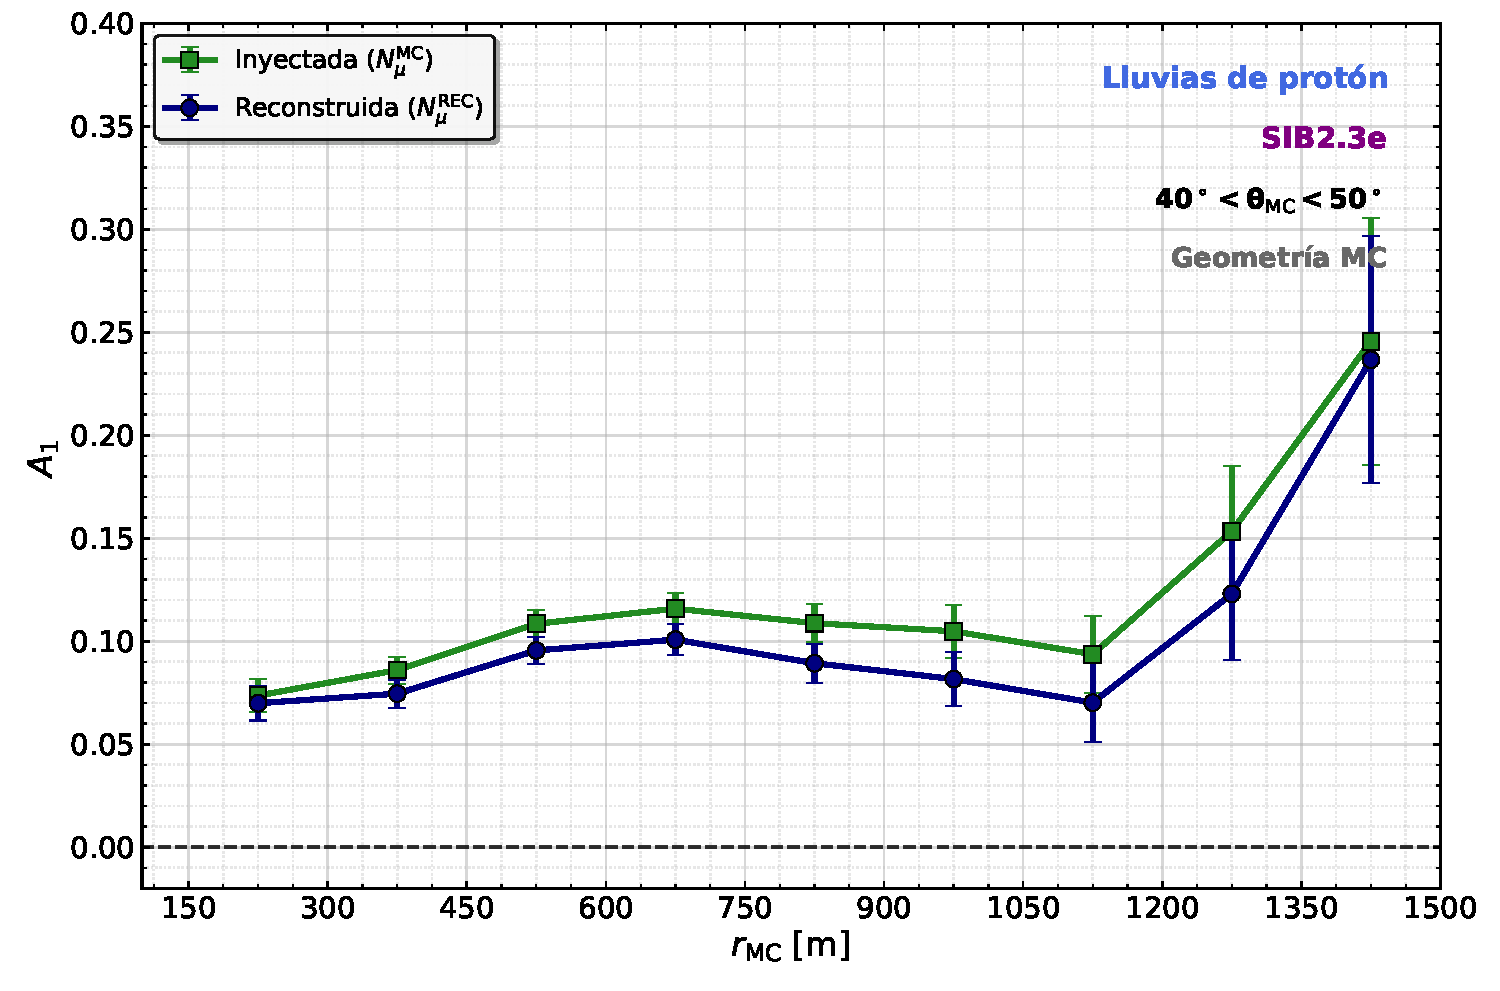
\includegraphics[width=\textwidth]{UMD_Asymmetry_MC_vs_REC.pdf}
    \column{0.37\textwidth}
      \begin{itemize}
        \item $40^\circ$--$50^\circ$, true core and direction.
        \item Reconstructed muon number lowers $A_1$ by 5--23\%, same shape.
        \item A separate effect from the core shift.
      \end{itemize}
  \end{columns}
\end{frame}

\begin{frame}{Backup: the counting bias depends on azimuth}
  \badgeAD
  \begin{columns}[c]
    \column{0.49\textwidth}
      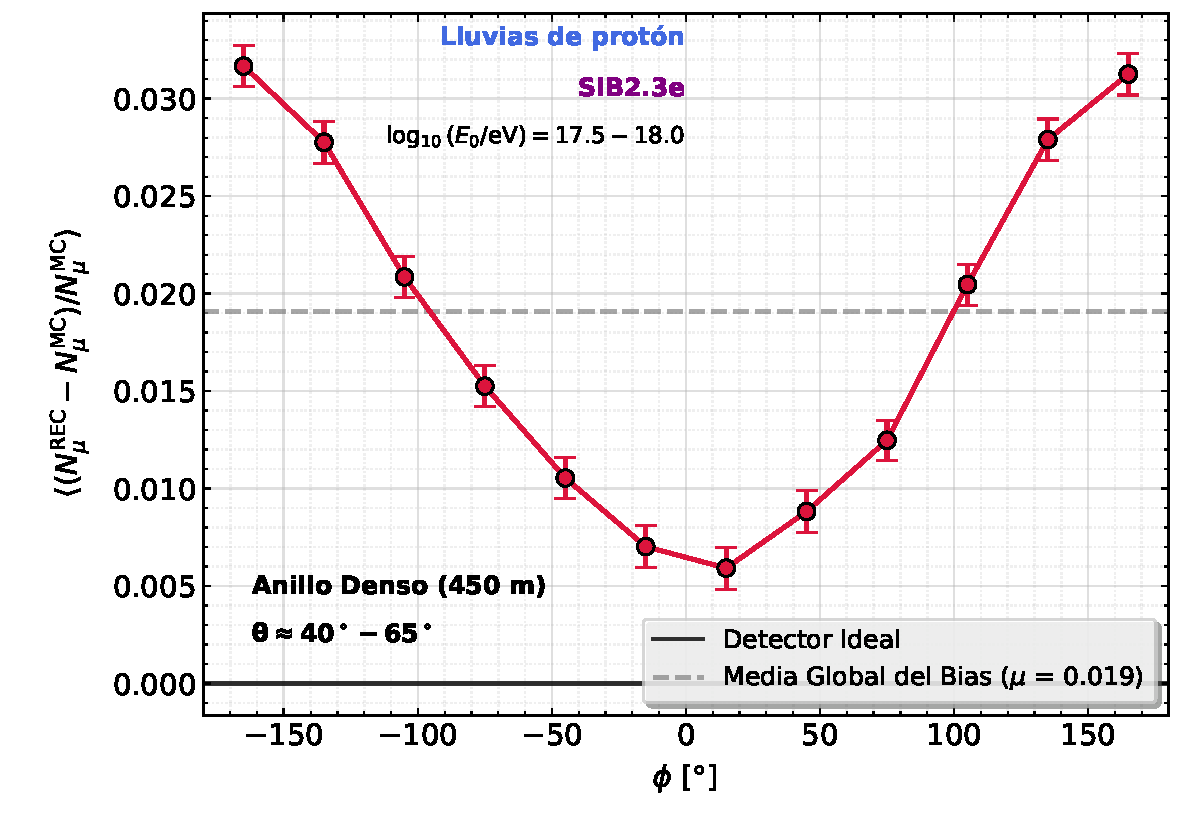
\includegraphics[width=\textwidth]{directional_bias.pdf}
    \column{0.49\textwidth}
      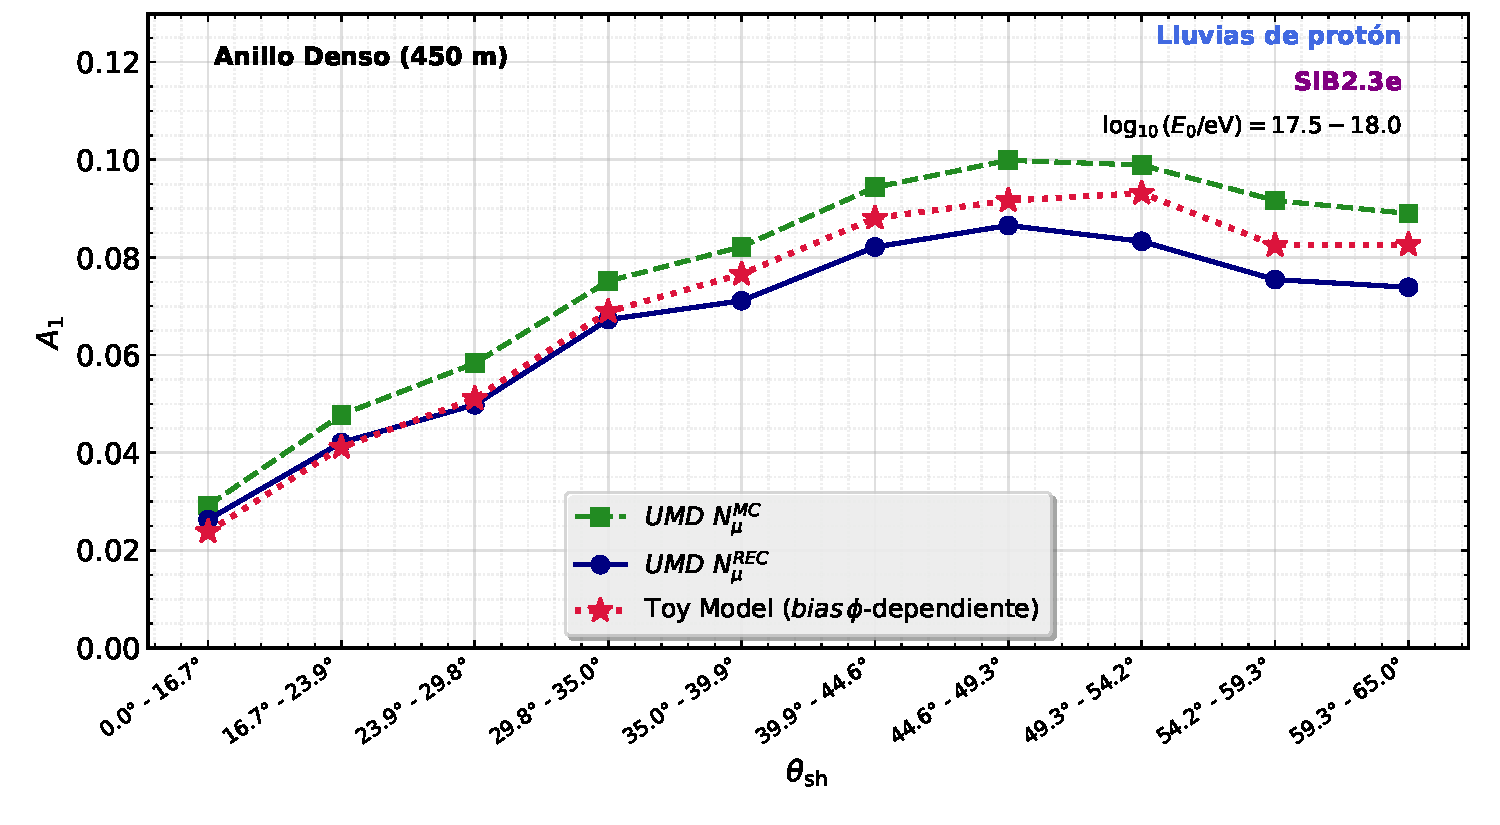
\includegraphics[width=\textwidth]{toy_model.pdf}
  \end{columns}
  \footnotesize
  \begin{itemize}
    \item Mean relative residual $(N^{\text{REC}}-N^{\text{MC}})/N^{\text{MC}}$ is larger
      on the late side (fewer muons) $\Rightarrow$ lower $A_1$.
    \item Bootstrap with the per-region residuals reproduces $A_1^{\text{REC}}$ up to
      $\theta\approx35^\circ$; above, half to two thirds of the loss. Remnant open.
  \end{itemize}
\end{frame}

\begin{frame}{Backup: fit grids, MC and REC geometry ($40^\circ$--$50^\circ$)}
  \badgeIF
  \begin{columns}[T]
    \column{0.5\textwidth}
      \centering\footnotesize MC geometry\\
      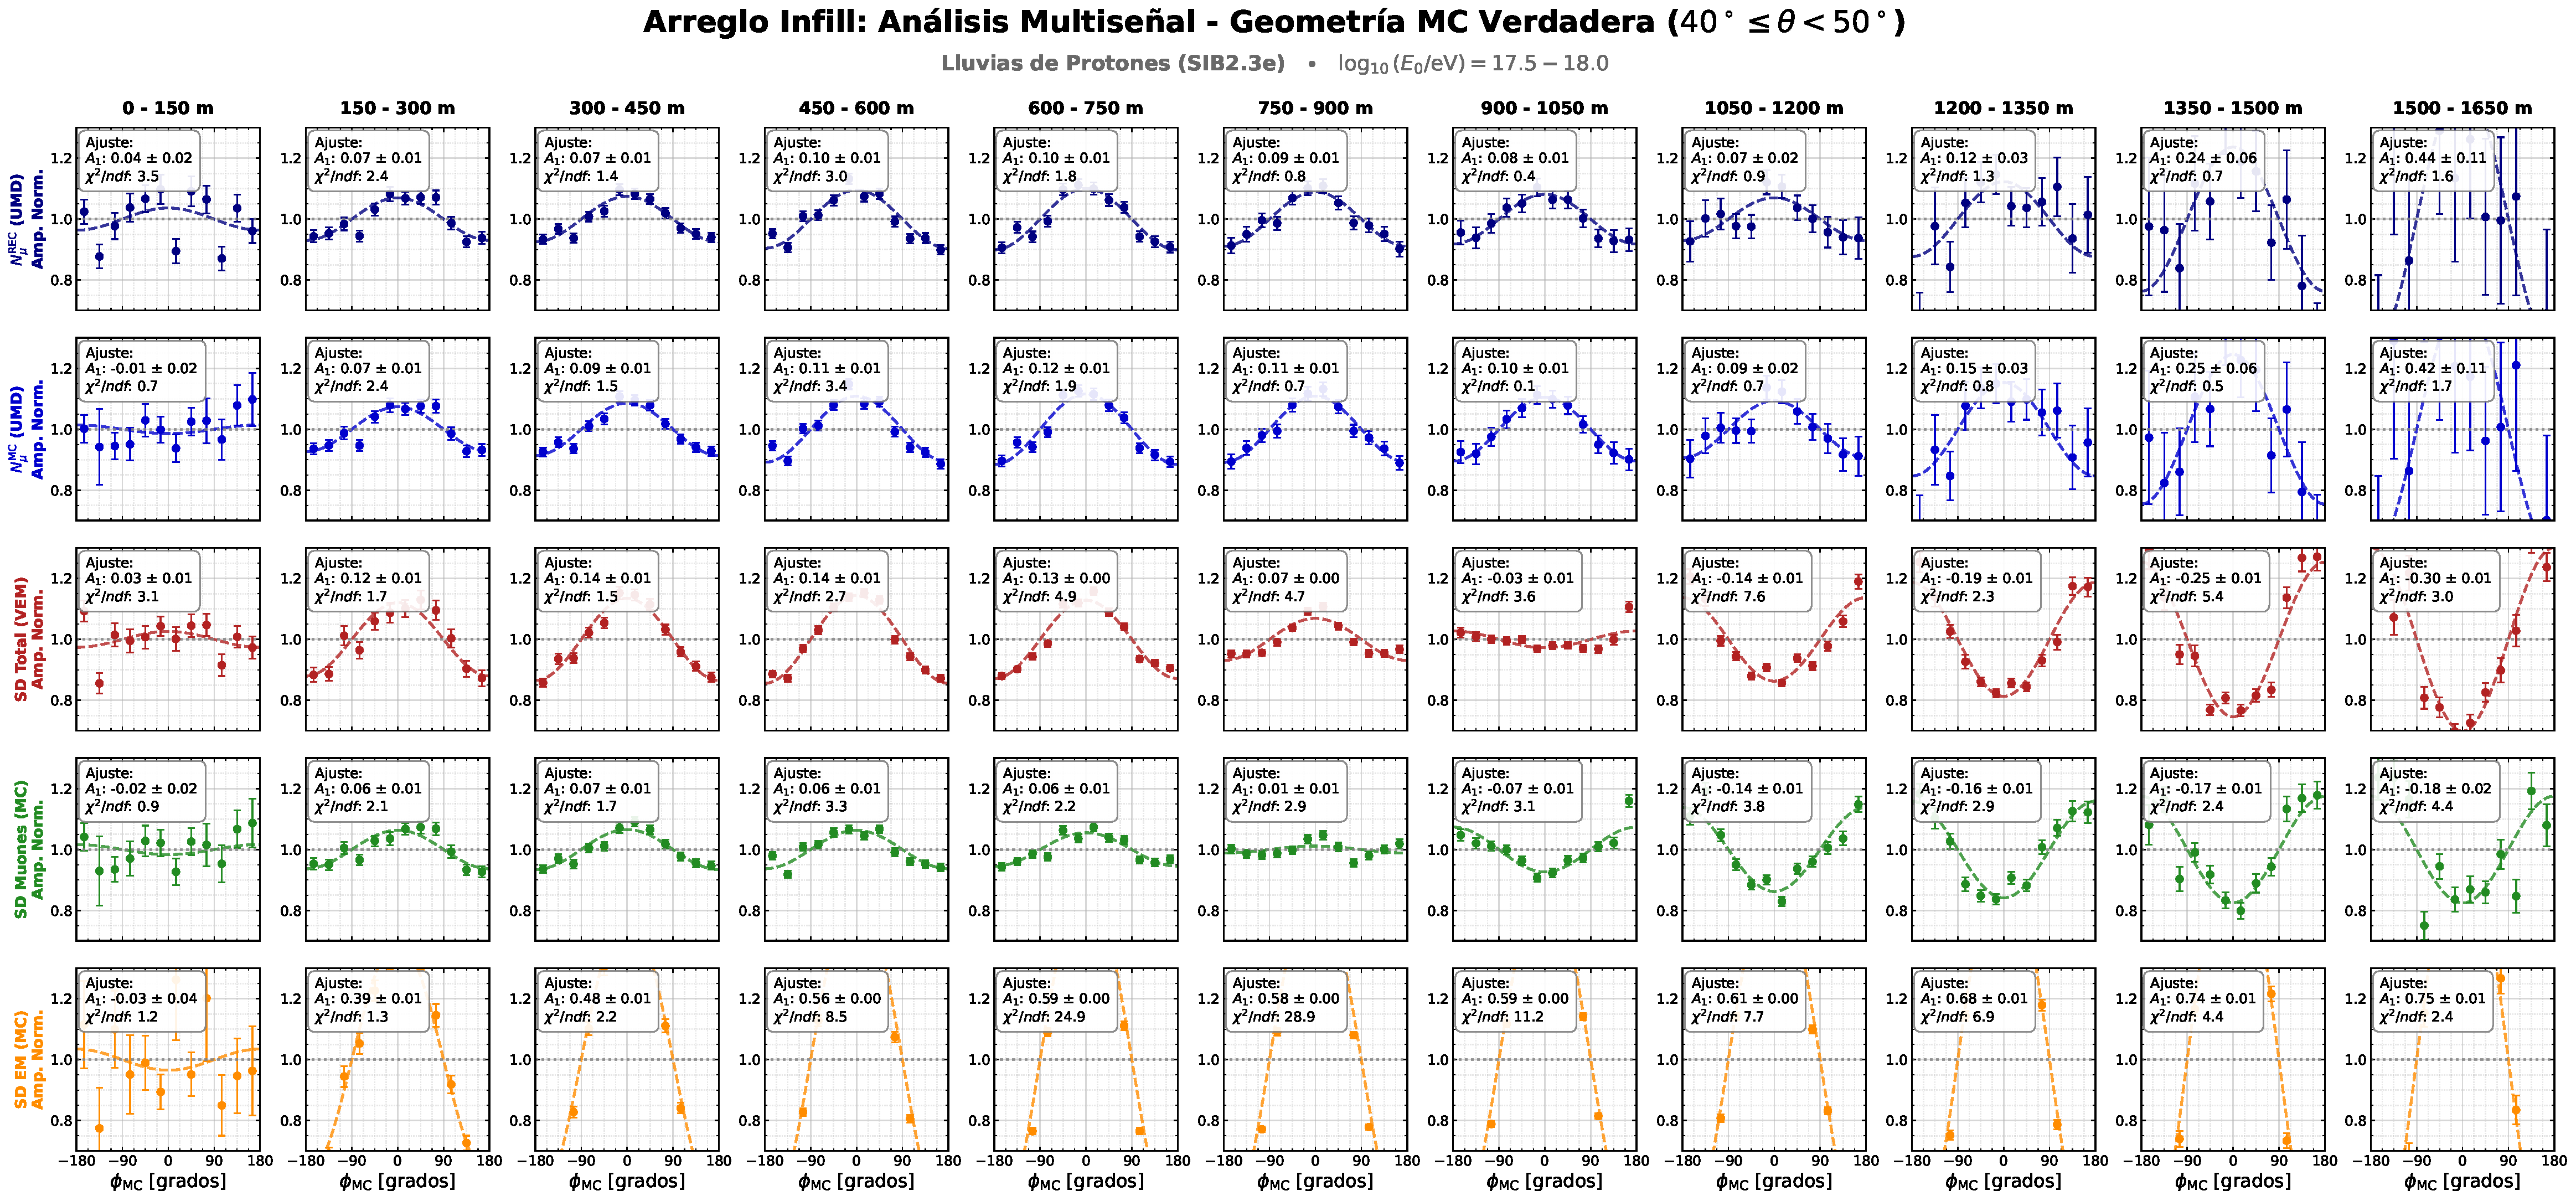
\includegraphics[width=\textwidth,height=5.6cm,keepaspectratio]{Anexo_Grilla_MC_40_50.pdf}
    \column{0.5\textwidth}
      \centering\footnotesize REC geometry\\
      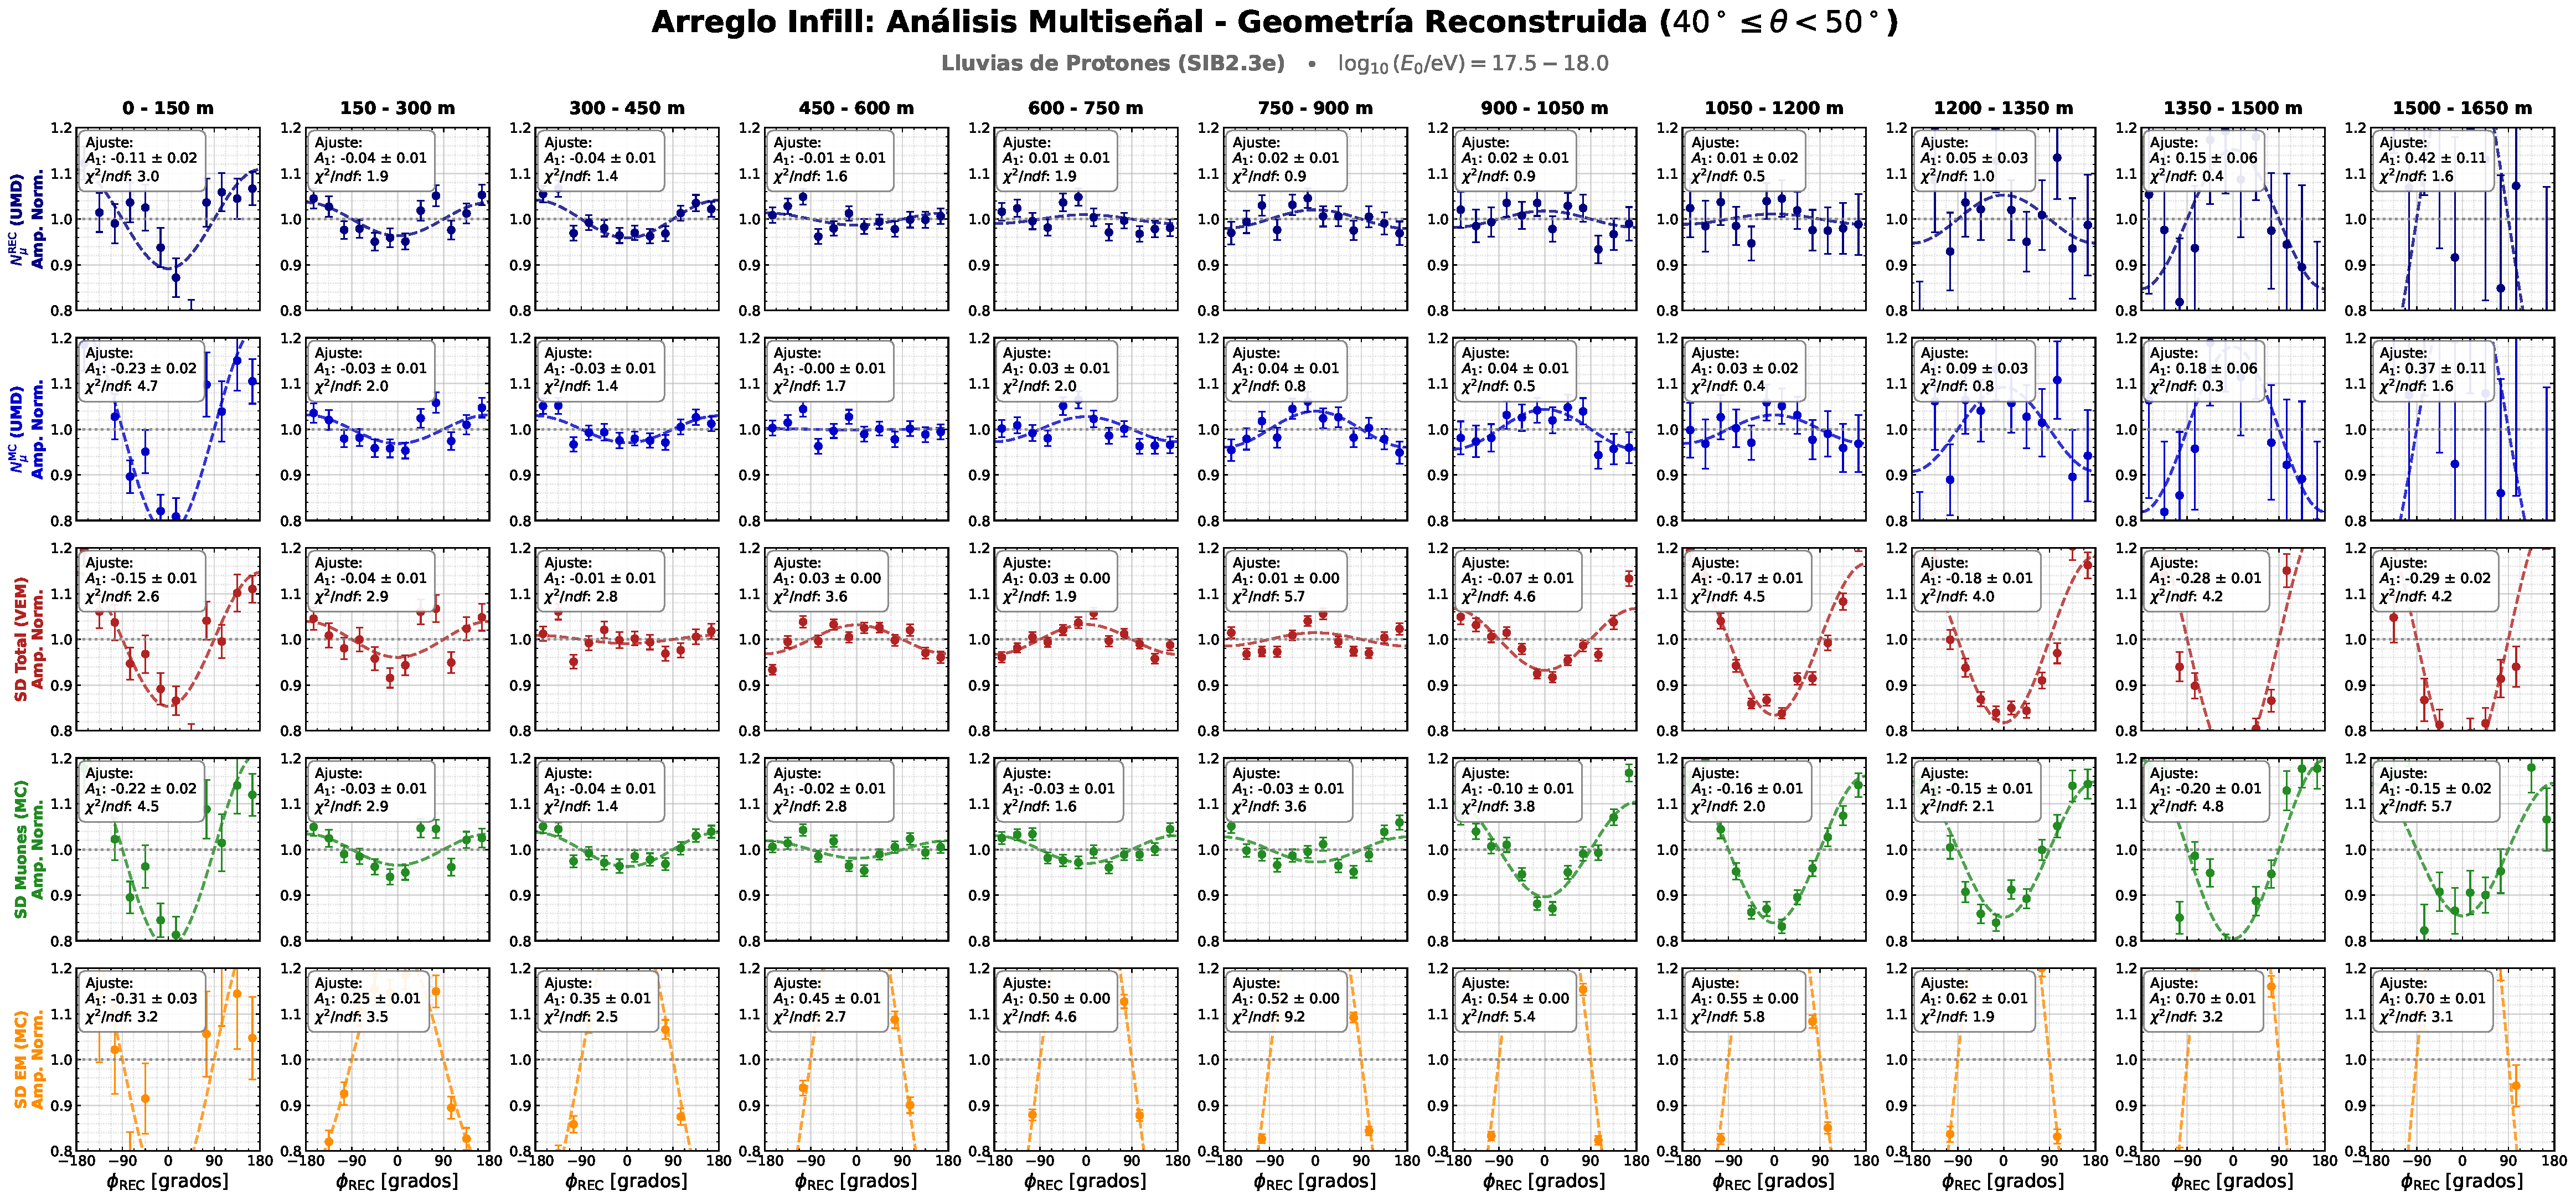
\includegraphics[width=\textwidth,height=5.6cm,keepaspectratio]{Anexo_Grilla_REC_40_50.pdf}
  \end{columns}
\end{frame}

\begin{frame}{Backup: fit quality on the Dense Ring}
  \badgeAD
  \begin{columns}[c]
    \column{0.60\textwidth}
      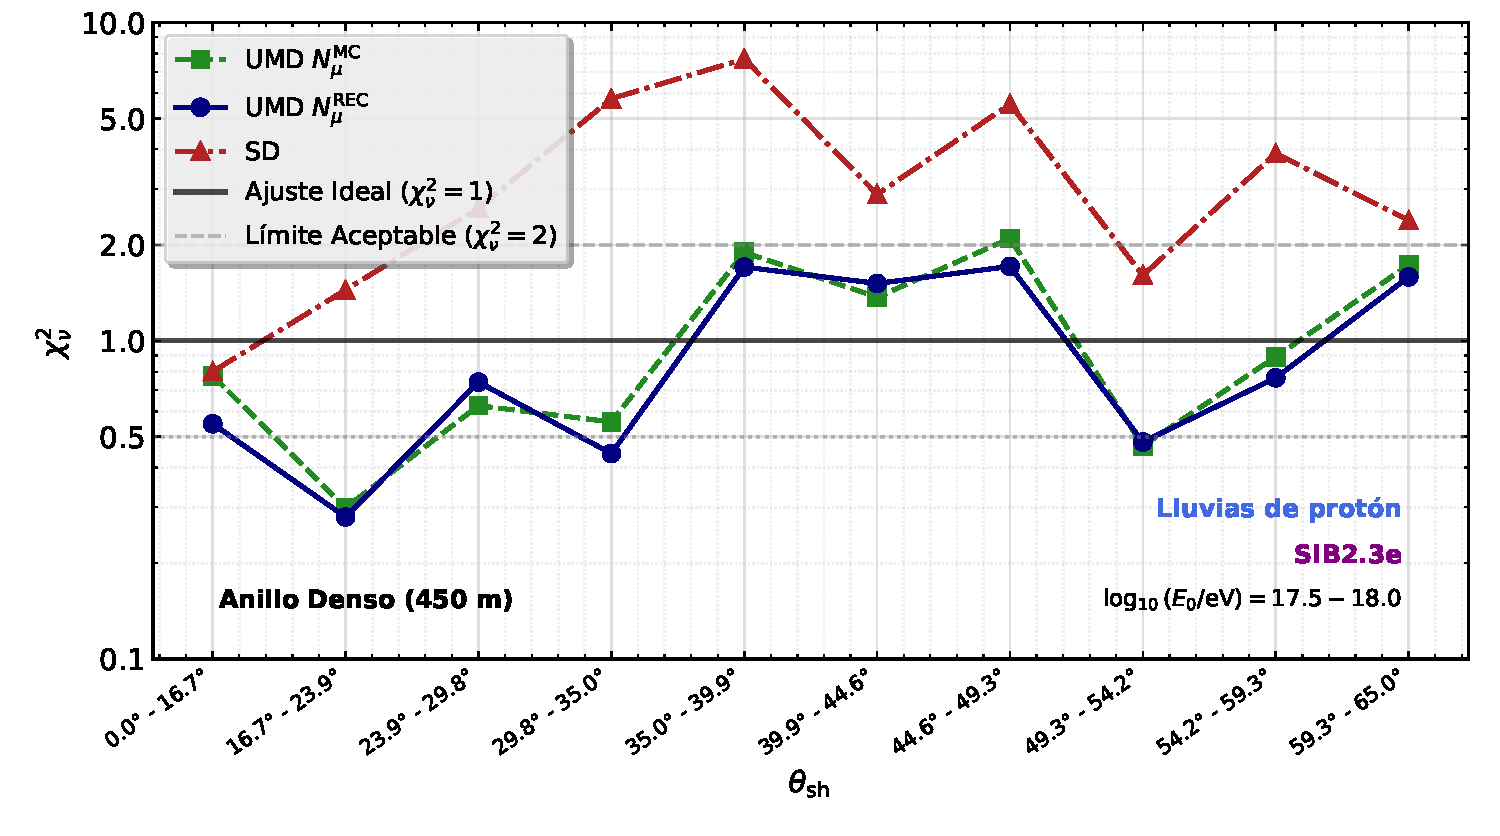
\includegraphics[width=\textwidth]{Chi2_Reduced_Fits.pdf}
    \column{0.37\textwidth}
      \begin{itemize}
        \item UMD, MC and REC: $\chi^2_\nu\approx1$.
        \item SD: $\chi^2_\nu$ up to $\sim10$; with such small errors the fit is
          sensitive to higher harmonics and to correlations between stations of
          one shower.
      \end{itemize}
  \end{columns}
\end{frame}

\begin{frame}{Backup: robustness}
  \badgeAD
  \begin{columns}[T]
    \column{0.49\textwidth}
      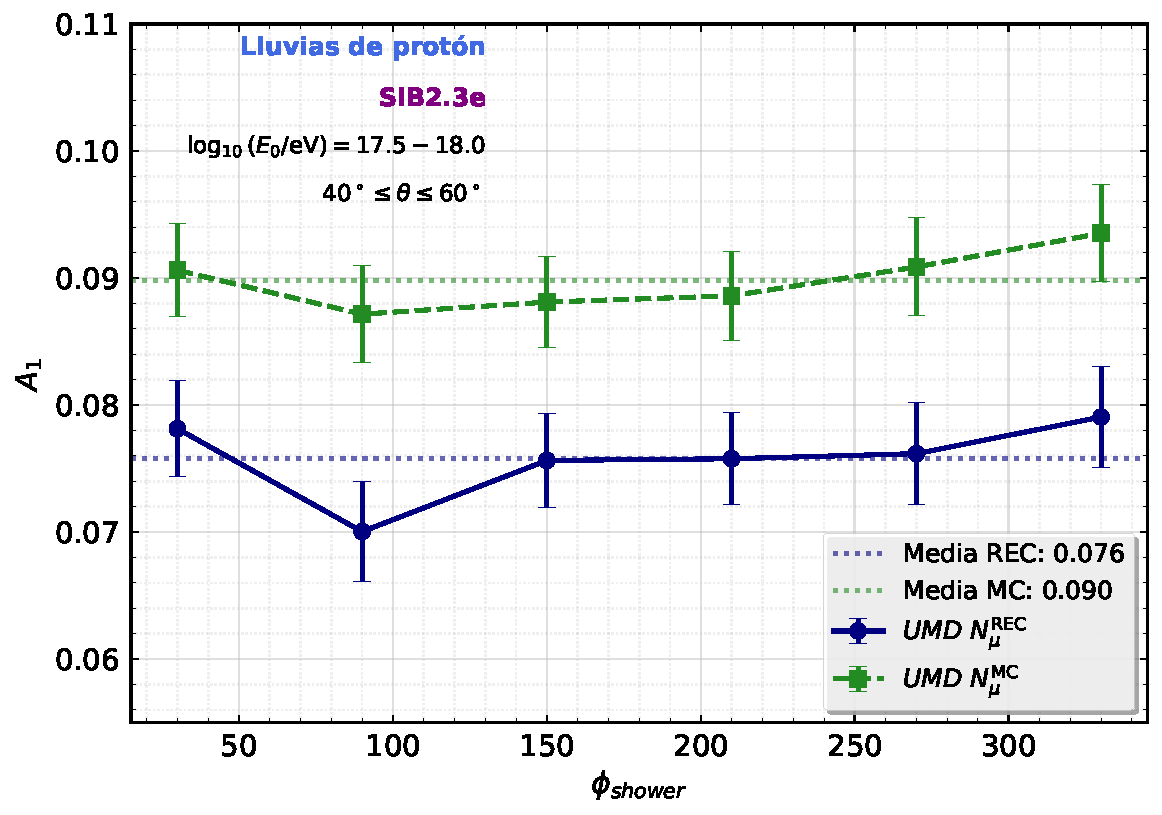
\includegraphics[width=\textwidth]{DenseRing_Systematics_Isotropy.pdf}
      \footnotesize Independent of the shower arrival azimuth ($40$--$60^\circ$).
    \column{0.49\textwidth}
      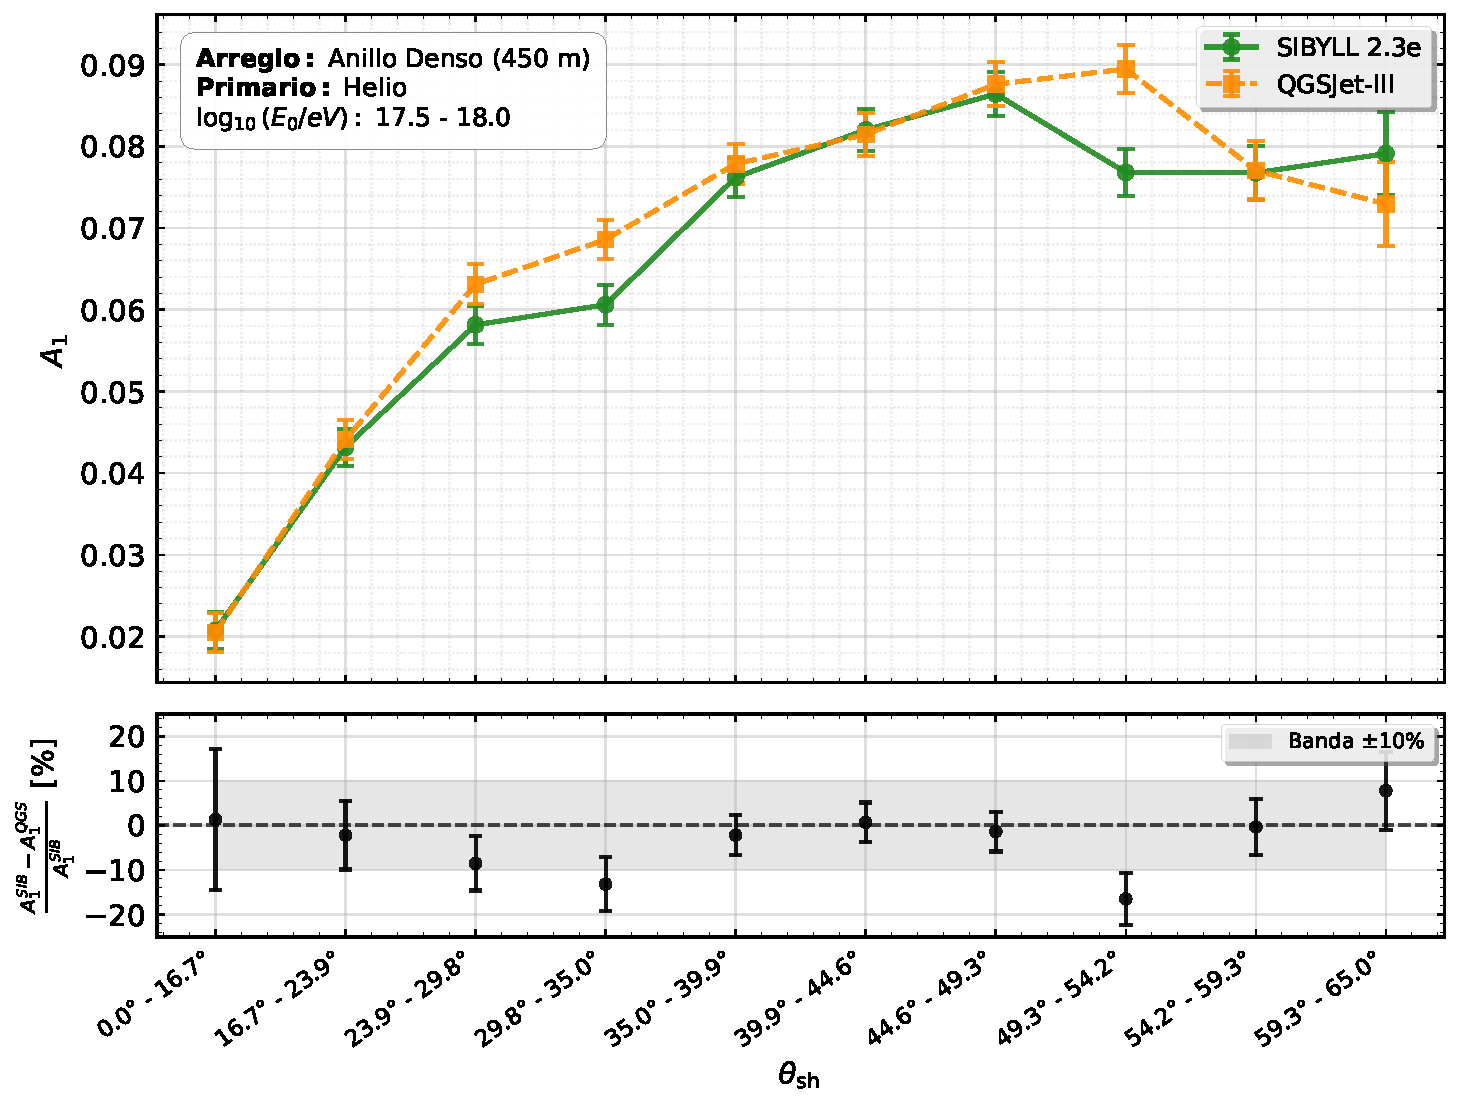
\includegraphics[width=\textwidth]{Hadronic_Uncertainty_Helium.pdf}
      \footnotesize Helium: SIBYLL~2.3e vs.\ QGSJET-III within $\pm10\%$ over most of
      the range.
  \end{columns}
\end{frame}

\begin{frame}{Backup: reconstruction performance}
  \begin{columns}[T]
    \column{0.33\textwidth}
      \centering
      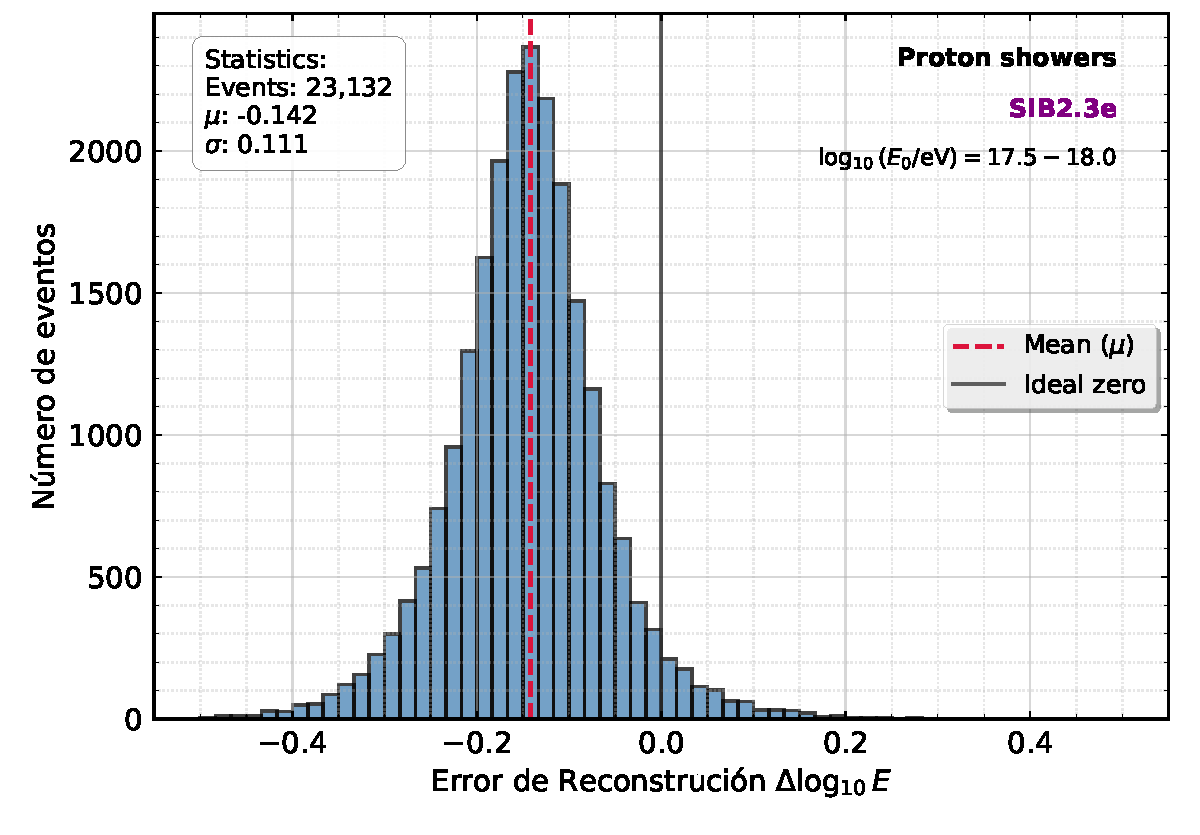
\includegraphics[width=\textwidth]{energy_bias.pdf}
    \column{0.33\textwidth}
      \centering
      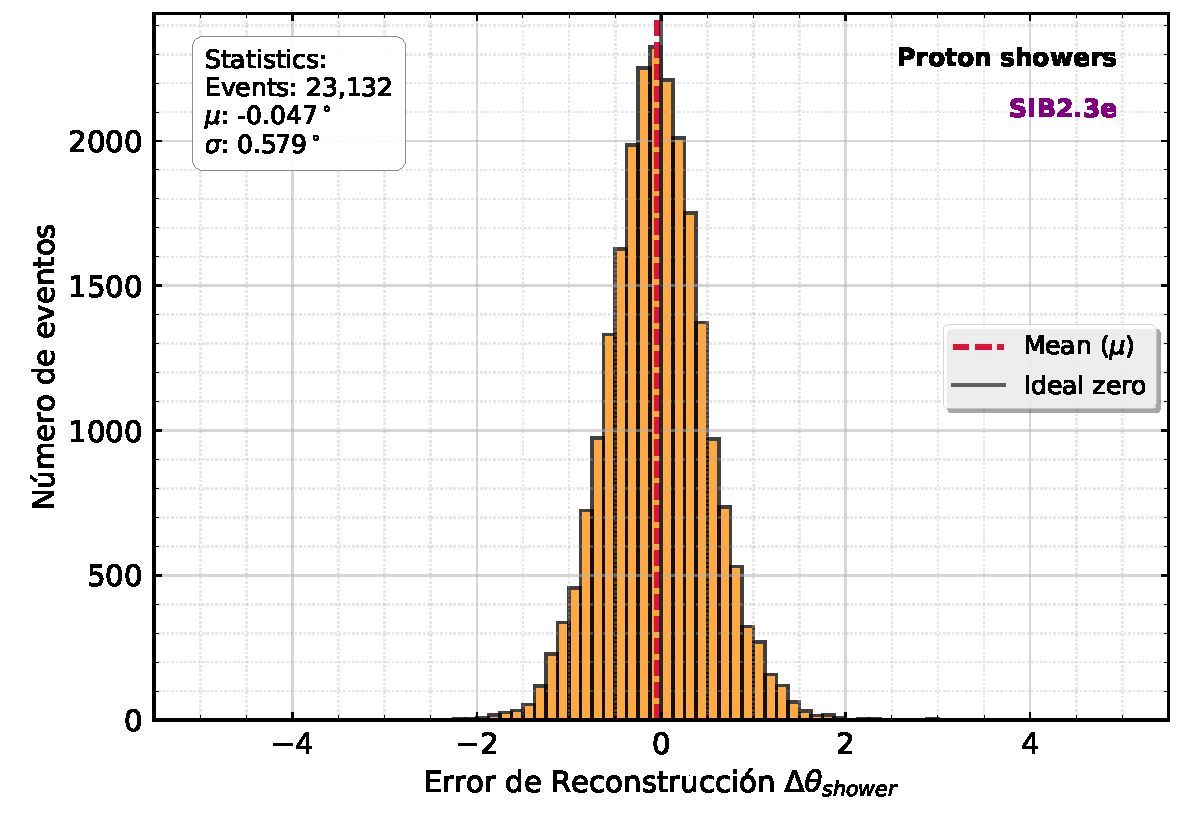
\includegraphics[width=\textwidth]{theta_bias.pdf}
    \column{0.33\textwidth}
      \centering
      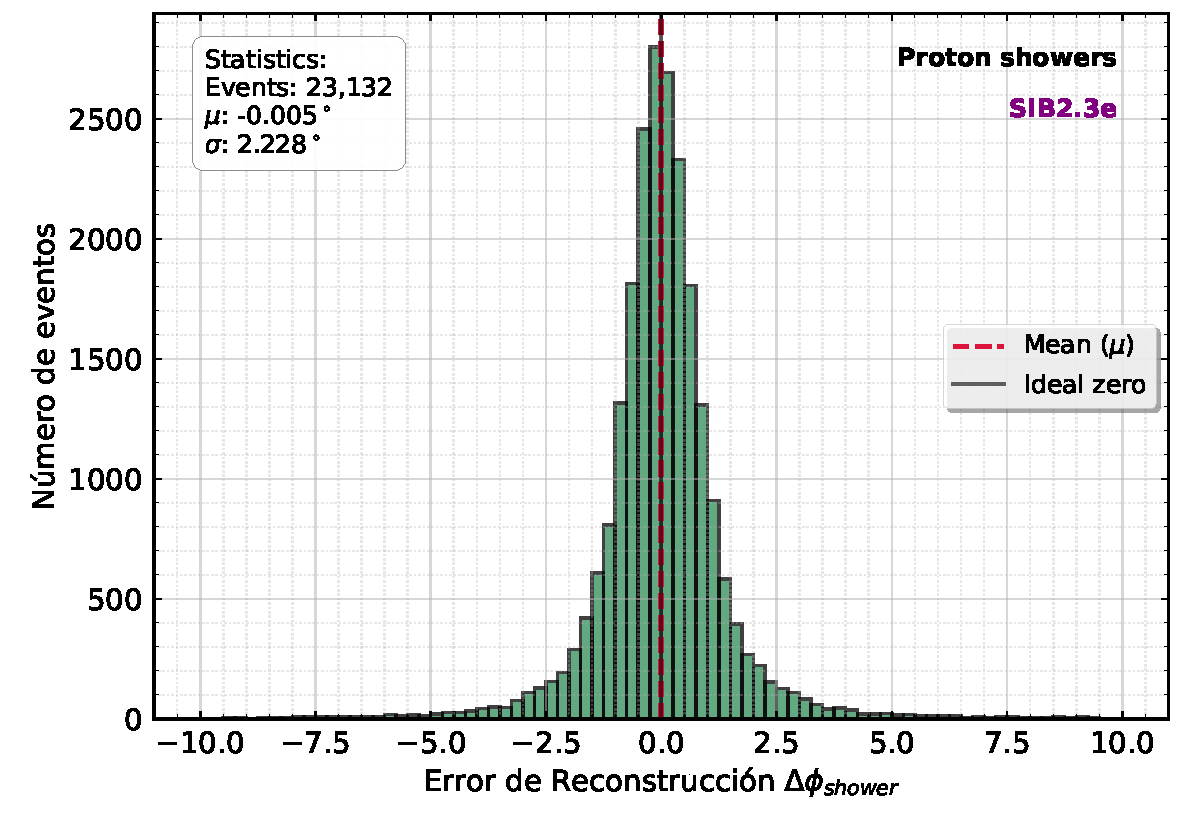
\includegraphics[width=\textwidth]{phi_bias.pdf}
  \end{columns}
  \small
  \begin{itemize}
    \item Energy: $\mu\approx-0.142$, $\sigma\approx0.111$ in $\Delta\log_{10}E$.
    \item $\theta$: bias $-0.05^\circ$, $\sigma=0.58^\circ$. $\phi$: bias
      $-0.005^\circ$, $\sigma=2.2^\circ$.
  \end{itemize}
\end{frame}

\begin{frame}{Backup: why the core shift does not affect the Dense Ring}
  \badgeAD
  \begin{itemize}
    \setlength{\itemsep}{0.5em}
    \item The ring stations are placed during the simulation at 450~m from the
      \textbf{true} axis: the shifted core does not make the ring eccentric.
    \item It only rotates the azimuth assigned to each station, by
      $\sim b/r\approx2^\circ$, much less than the $30^\circ$ spacing.
    \item It affects $N_\mu^{\text{MC}}$ and $N_\mu^{\text{REC}}$ in the same way, so
      it cannot explain the MC--REC gap on the ring (that gap is the counting bias).
  \end{itemize}
\end{frame}

\begin{frame}{Backup: field data (preliminary)}
  \badgeDATA
  \vspace{-0.8em}
  \begin{columns}[c]
    \column{0.60\textwidth}
      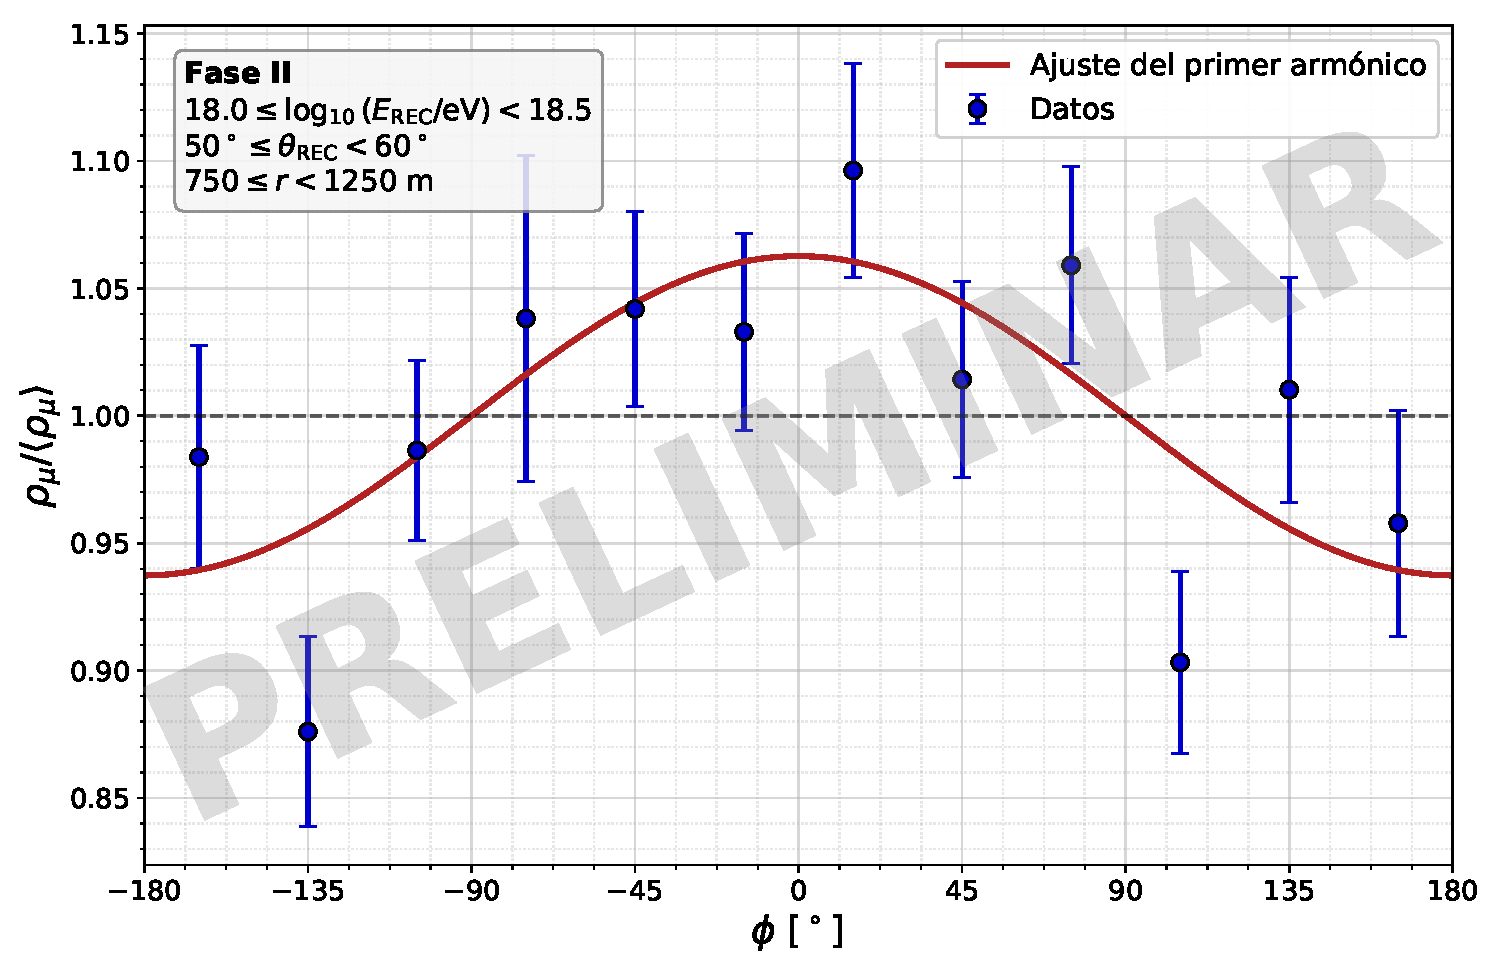
\includegraphics[width=\textwidth]{datos_campo_preliminar.pdf}
    \column{0.38\textwidth}
      \footnotesize
      \setbeamerfont{itemize/enumerate body}{size=\footnotesize}
      \begin{itemize}
        \item UMD muon density vs.\ $\phi$, normalized to its mean; Phase~II, cuts in
          the box.
        \item Maximum at $\phi\approx0$: \textbf{early excess}, as in the
          simulations.
        \item \textbf{Preliminary}: no core-shift correction, no systematics, no MC
          above $10^{18}$~eV for this bin.
      \end{itemize}
  \end{columns}
\end{frame}

\begin{frame}{Backup: $A_1(r)$ in field data vs.\ simulations}
  \badgeDATA
  \vspace{-0.8em}
  \centering
  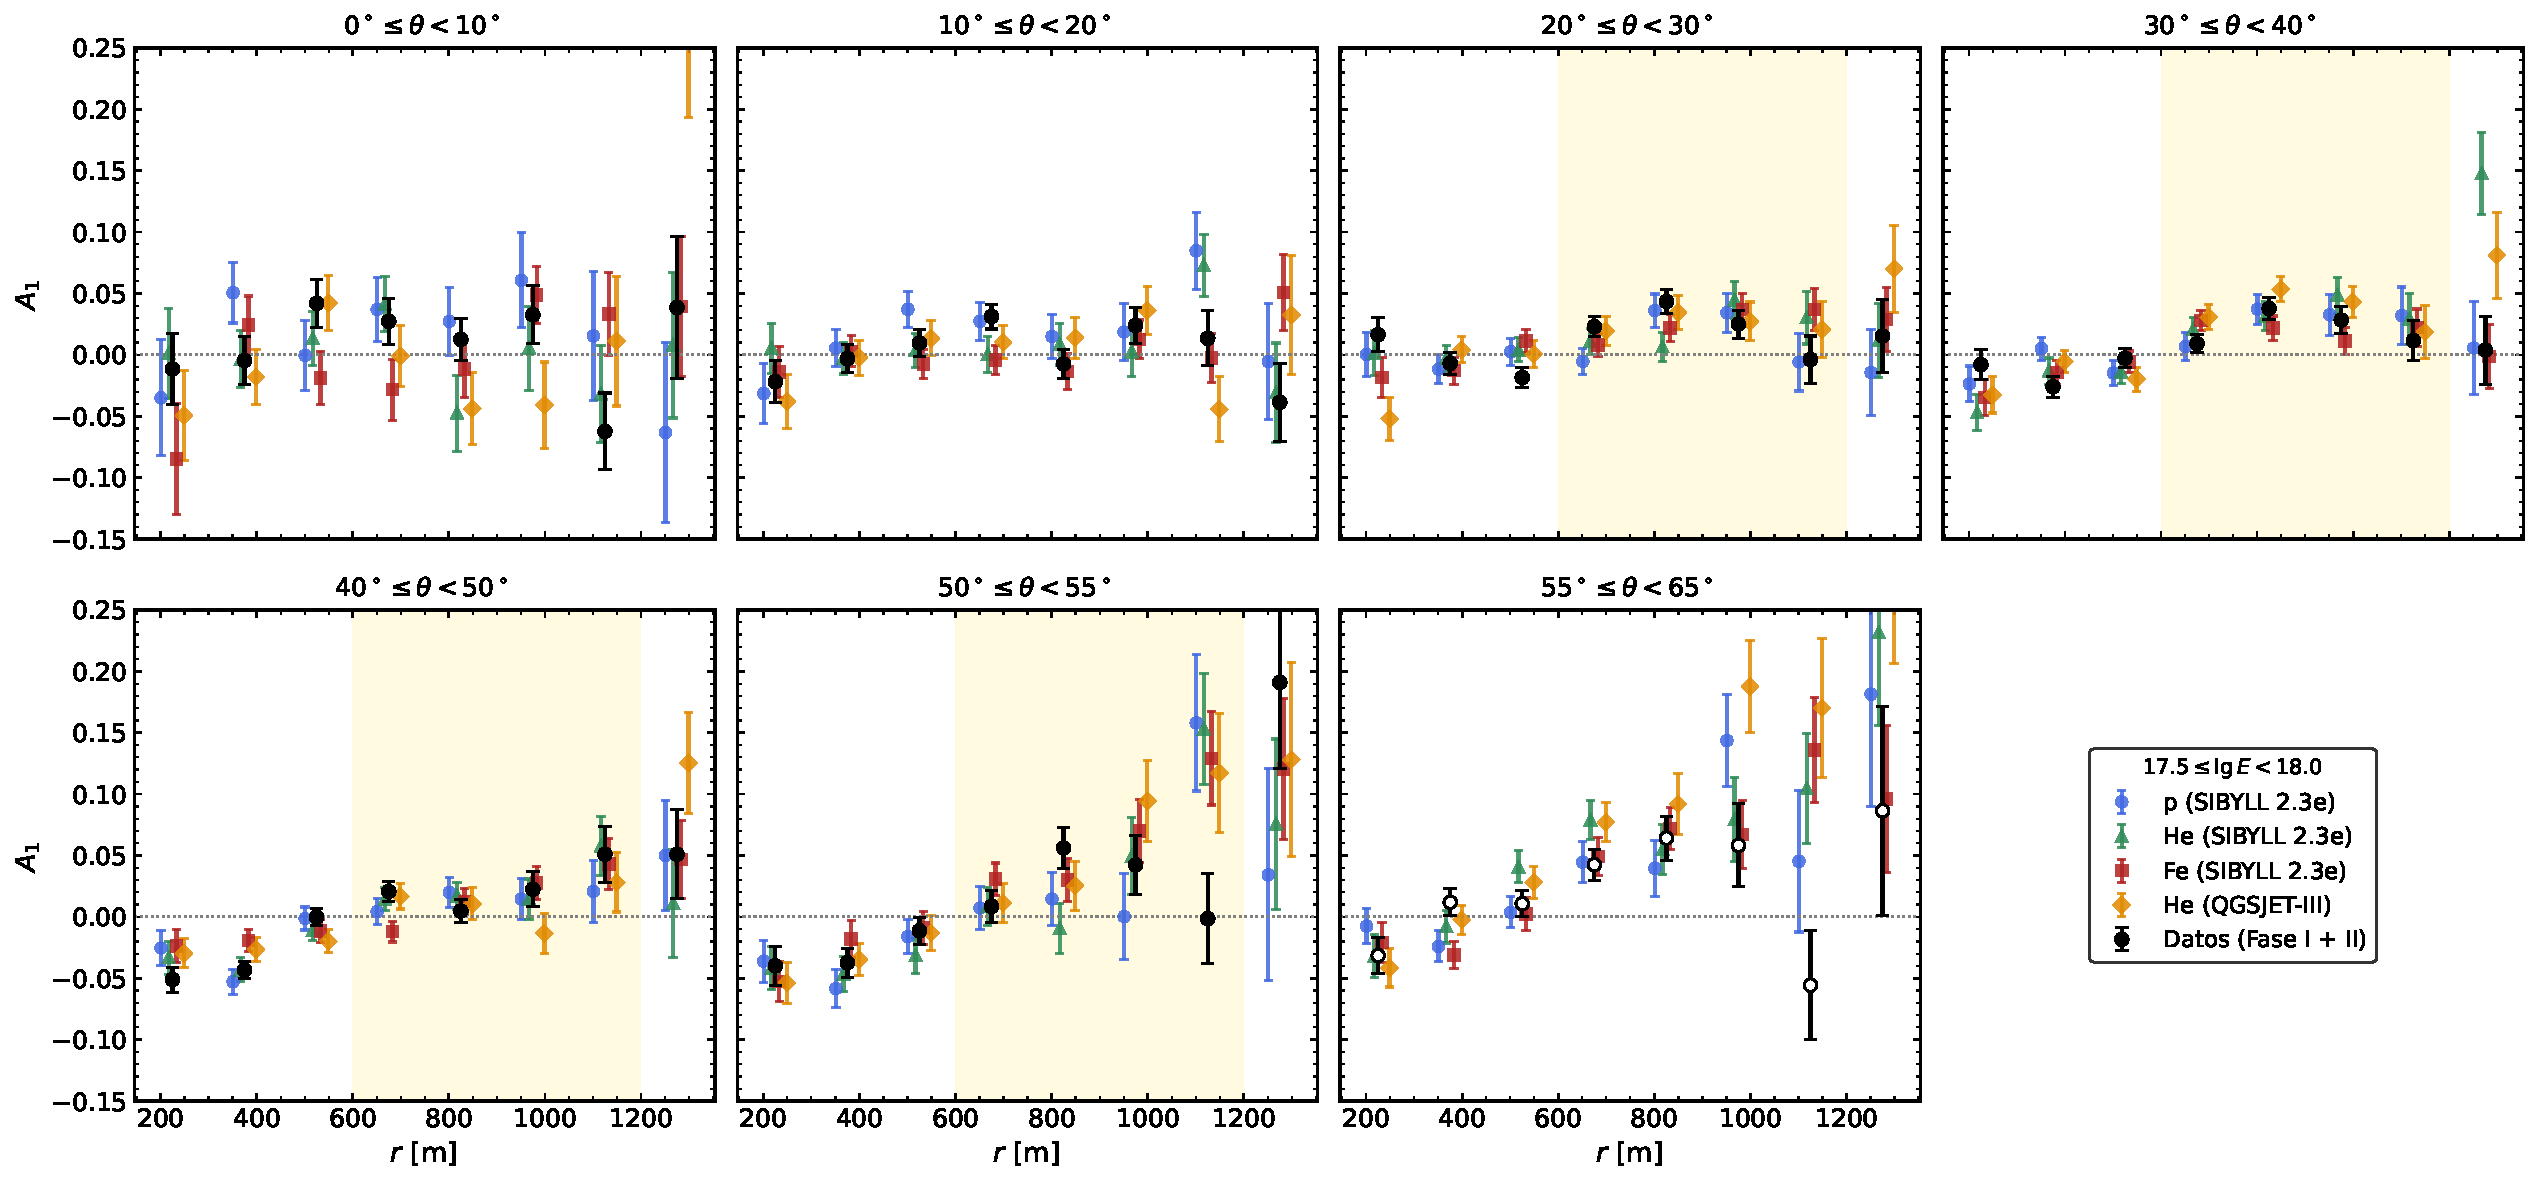
\includegraphics[width=\textwidth,height=5.6cm,keepaspectratio]{cap7_A1_vs_r_datos_vs_mc.pdf}

  \footnotesize UMD Infill, Phase~I + Phase~II, 6T5, $17.5\le\lg(E/\text{eV})<18.0$, REC
  geometry in data and simulations.
\end{frame}

\end{document}
